\documentclass[10pt, a4paper, oneside]{article}
\usepackage[hidelinks]{hyperref}
\usepackage{jucs2e}
\usepackage{graphicx}
\usepackage{url}
\usepackage{ulem}
\usepackage{mathtools}
\usepackage{scalerel}
\usepackage{setspace}
\usepackage[strict]{changepage}
\usepackage{caption}
\usepackage[letterspace=-50]{microtype}
\usepackage{fontspec}
\usepackage{afterpage}
\usepackage{ragged2e}
\usepackage{multicol, multirow}
\usepackage{makecell}
\usepackage{amsfonts}

\setmainfont{Times New Roman}

\usepackage{titlesec}

\titleformat*{\section}{\Large\bfseries}
\titleformat*{\subsection}{\normalsize\bfseries}

\renewcommand{\baselinestretch}{0.9} 

\graphicspath{{./figures/}}

\usepackage[textwidth=8cm, margin=0cm, left=4.6cm, right=4.2cm, top=3.9cm, bottom=6.8cm, a4paper, headheight=0.5cm, headsep=0.5cm]{geometry}
\usepackage{fancyhdr}
\usepackage[format=plain, labelfont=it, textfont=it, justification=centering]{caption}
\usepackage{breakcites}
\usepackage{microtype}
 
\apptocmd{\frame}{}{\justifying}{}


\urlstyle{same}
\pagestyle{fancy}

\newcommand\jucs{{Journal of Universal Computer Science}}
\newcommand\jucsvol{vol. 31, no. 14 (2025)}
\newcommand\jucspages{1583-1606}     
\newcommand\jucssubmitted{4/12/2024}
\newcommand\jucsaccepted{25/5/2025}
\newcommand\jucsappeared{28/12/2025}
\newcommand\jucslicence{ CC BY 4.0}
\newcommand\startingPage{1583}
\setcounter{page}{\startingPage}

%Author
\newcommand\paperauthor{{Phuong N.T.H., Nhat P.M., Hieu N.V.:}}

% Title
\newcommand\papertitle{NirMACNet: A Novel Multi-Scale Adaptive Convolutional Network for NIR Spectroscopy}

% Main header content
\header{\paperauthor \papertitle}

\begin{document}

\title{{\fontsize{14pt}{14pt}\selectfont{\vspace*{-3mm}\papertitle\vspace*{-1mm}}}}

\author{{\bfseries\fontsize{10pt}{10pt}\selectfont{Nguyen Thi Hoang Phuong}} \\
   {\fontsize{9pt}{12pt}\selectfont{(Pham Van Dong University Viet Nam, Quang Ngai, VietNam\\
   \orcid{0009-0009-6755-604X}, 
   nthphuong@pdu.edu.vn)}}
   \and
   {\bfseries\fontsize{10pt}{10pt}\selectfont{Phan Minh Nhat}}\\
   {\fontsize{9pt}{12pt}\selectfont{(The University of Danang - University of Science and Technology, Danang, Vietnam \\
   \orcid{0009-0008-3861-9892}, 
   nhat0299@gmail.com)}}
   \and
   {\bfseries\fontsize{10pt}{10pt}\selectfont{Nguyen Van Hieu}}\\
   {\fontsize{9pt}{12pt}\selectfont{(The University of Danang - University of Science and Technology, Danang, Vietnam \\
   \orcid{0000-0001-5311-806X},  
   nvhieuqt@dut.udn.com)}}
}

\label{first}
\maketitle

{\fontfamily{ptm}\selectfont
\begin{abstract}
{\fontsize{9pt}{9pt}\selectfont{\vspace*{-2mm}
Near-infrared (NIR) spectroscopy has emerged as a valuable analytical technique for assessing the composition and quality of various materials. This study proposes NirMACNet, a novel convolutional neural network (CNN) architecture that incorporates a residual-based multiscale kernel mechanism for enhanced prediction of compositional attributes. The model is evaluated on two distinct NIR spectral datasets, milk and soil, to demonstrate its generalization capability across domains. By leveraging multiscale kernel operations, NirMACNet effectively captures diverse spectral patterns, while its deep architecture facilitates comprehensive feature extraction. To mitigate performance degradation commonly associated with deeper networks, residual learning is employed. Experimental results indicate that NirMACNet consistently outperforms state-of-the-art methods in terms of prediction accuracy. Future work will involve expanding the diversity of training datasets and investigating alternative architectural enhancements to further improve model robustness and applicability.}}
\end{abstract}}

{\fontfamily{ptm}\selectfont
\begin{keywords}
{\fontsize{9pt}{9pt}\selectfont{Near infrared spectroscopy, Food product analysis, Multi-scale feature extraction, Deep Learning, NirMACNet}}
\end{keywords}}

{\fontfamily{ptm}\selectfont
\begin{category}
{\fontsize{9pt}{9pt}\selectfont{
H.3.1, H.3.2, H.3.3, H.3.7, H.5.1}}
\end{category}}

{\fontfamily{ptm}\selectfont
\begin{doi}
{\fontsize{9pt}{9pt}\selectfont{
10.3897/jucs.143527}}
\end{doi}}

\section{Introduction}
Accurate characterization of the chemical composition of raw materials and agricultural products is essential across various industries, including food processing, pharmaceuticals, agriculture, and environmental monitoring. These materials often consist of complex mixtures whose compositional attributes, such as moisture, protein, fat, or mineral content, significantly influence their quality, functionality, and economic value. Conventional analytical methods, such as chromatography and wet chemistry, though precise, are often labor-intensive, time-consuming, and require extensive sample preparation. In contrast, near-infrared (NIR) spectroscopy has emerged as a rapid, non-destructive, and cost-effective alternative for assessing the composition of a wide range of materials. However, the spectral variability inherent in different sample types, combined with the high dimensionality and overlapping absorption bands of NIR data, poses significant challenges for accurate modeling. To address these challenges, this study introduces a deep learning-based approach for predicting compositional attributes from NIR spectra, with the aim of improving generalizability and predictive accuracy across diverse material domains.

Chemometrics, a discipline that leverages artificial intelligence (AI) for chemical analysis, has prominently featured the value of "chemical" and "analytical" intelligence for decades through studies by \cite{marini2009artificial}, and \cite{marini2008artificial}. While artificial neural networks (ANNs) have found application in chemometrics as cited in a study by \cite{debus2021deep}, their advantages over established techniques like partial least squares (PLS) for classification and prediction have been limited. Recent studies by  \cite{cui2018modern}, \cite{ng2020influence}, \cite{ng2019convolutional}, \cite{mishra2021synergistic}, and \cite{einarson2022predicting}, however, demonstrate the potential of deep learning (DL) to surpass PLS in predictive power using NIR spectroscopic data. \cite{anderson2020achieving} have found that NIR spectra represent a combination of linear and non-linear molecular vibrations alongside physical effects like light scattering baselines and path-length variations. Classical chemometrics, particularly principal component analysis (PCA) and PLS with knowledge-driven pre-processing have achieved success in NIR data modeling. However, to address data non-linearities and enhance model performance, non-linear methods have been explored by \cite{smits1994using}. These methods, such as kernel support vector machines, can suffer from overfitting due to their lack of inherent regularisation (unbounded degrees of freedom) as cited in a study by \cite{melssen1994using}. While traditional ANNs have a long history in chemometrics, they differ significantly from recent deep learning architectures. Traditional ML algorithms, including ANNs, require pre-extracted features from spectra as input. In contrast, DL models can automatically learn feature extraction, potentially incorporating spectroscopic pre-processing steps as cited in works by \cite{acquarelli2017convolutional}, and \cite{helin2022possible}. This allows DL to optimize models through both feature extraction and data-driven pre-processing. Additionally, DL architectures can integrate significantly more layers of various types compared to traditional ANNs, with the potential for training models with hundreds of layers and millions of parameters (potentially leading to overfitting). Advancements in computational power (GPUs), improved regularisation techniques, and sophisticated model optimization approaches have facilitated this capability. 

Traditional feature extraction methods for near-infrared (NIR) spectroscopy rely on prior knowledge and are often task-specific. This approach becomes increasingly laborious as NIR data complexity and diversity grow, requiring a dedicated feature extractor for each unique data type. Studies by \cite{zhu2015hierarchical}, and \cite{takanobu2019hierarchical} have pointed out that deep learning offers a compelling alternative, enabling the direct extraction of high-level and hierarchical representations from large datasets. Convolutional Neural Networks (CNNs) of \cite{chakravartula2022use}, Deep Belief Networks (DBNs) of \cite{guindo2021potential}, and \cite{yang2017deep}, Residual CNNs (ResCNNs) of \cite{chen2022rapid}, and stacked Autoencoders (SAEs) of \cite{zihao2020near} are prominent deep learning architectures employed for various NIR analysis applications. 

NIR spectra data present a challenge for deep learning models due to their inherent characteristics. These data typically consist of long, one-dimensional (1-D) complex signals. Analyzing composition via NIR spectroscopy further necessitates the extraction of deeper and more intricate features to account for varying conditions. While deep 1-D architectures are suitable for this purpose, research has identified limitations associated with increasing network depth. Studies by \cite{srivastava2015highway}, \cite{he2015convolutional} report that accuracy tends to saturate and degrade beyond a certain point, independent of overfitting. This suggests that deeper networks might exacerbate performance degradation. Additionally, traditional deep networks utilize fixed-size convolutional kernels and pooling operations, which limit their ability to analyze data containing multi-scale features. Consequently, while deep learning offers significant advantages for data analysis, its effectiveness in extracting features from multi-scale NIR spectra data requires further exploration.

This paper introduces the NirMACNet architecture, a novel approach to address the limitations of existing methods in predicting milk composition. The key contributions of this work are highlighted as follows:
\begin{enumerate}
    \item  The NirMACNet architecture, which leverages deep learning, is proposed for predicting composition in various materials. The model utilizes multi-scale convolutional kernels to extract features from raw NIR spectra across different scales. This multi-scale feature extraction enhances the model's robustness and ability to represent the captured characteristics, even under non-ideal measurement conditions. Furthermore, the architecture incorporates residual connections to facilitate learning in profound networks, specifically addressing the performance degradation issue observed in traditional deep learning models for NIR spectra analysis.
    \item  The NirMACNet architecture capitalizes on the strengths of CNNs for feature extraction and regression directly from raw NIR spectra data. This eliminates the need for complex preprocessing steps, streamlining the overall analysis process and potentially reducing the risk of information loss during preprocessing.
\end{enumerate}

\section{Related Work}\label{sec2}
\subsection{Application of Machine Learning and Deep Learning in NIR Spectrum-Related Problems}\label{sec2.1}
NIR spectroscopy offers a versatile analytical technique for various chemical analyses, including quality component analysis, chemical composition determination, qualitative/classification tasks, and waveshape analysis. Alongside these established approaches, machine learning (ML) has emerged as a powerful tool for NIR spectral data analysis due to its reliability and effectiveness.

Studies have explored the integration of ML models with chemometrics for NIR data analysis. For example, \cite{cozzolino2007effect} combined Principal Component Analysis (PCA) and Partial Least Squares (PLS) to assess the impact of temperature on wine NIR spectra and predict various chemical constituents. While demonstrating the influence of temperature and successful prediction of alcohol, sugar, pH, and tartaric acid in wine samples, the model's characterization of other parameters could be further refined according to \cite{zhang2022review}. Similarly, another study by \cite{ozdemir2018quantification} utilized PLS with chemometrics for rapid analysis of sterols in olive oil, but limitations were observed in quantifying individual fatty acids regarding to \cite{zhang2022review}.

NIR spectral data modeling techniques can be broadly categorized into unsupervised and supervised learning approaches. Deep learning (DL), a powerful subset of ML, can be tailored to both categories. CNNs are prominent examples for supervised learning tasks in NIR spectroscopy as evidenced by studies from \cite{cui2018modern}, \cite{malek2018one}, while unsupervised learning often utilizes autoencoder (AE)-based methods of \cite{yu2018deep}. DL has shown potential in various applications, including prediction by \cite{zhang2019deepspectra}, calibration transfer by \cite{mishra2021deep}, model updating by \cite{mishra2021realizing}, and spectral image processing by \cite{mishra2021gan}. However, despite promising initial results, DL methods in NIR spectroscopy lack systematic applicability studies. The linear nature of chemical information within NIR spectra often leads to the preference for simpler models like PLS. Recent advancements in chemometrics and the early success of DL applications have positioned DL as a new tool with significant promise, although some researchers view its complexity as a potential drawback.

\subsection{Residual Learning}
NIR spectroscopy data present a challenge for deep learning models due to their inherent characteristics. These data typically consist of long, one-dimensional (1-D) complex signals. Additionally, the variability introduced by fluctuating operational conditions during NIR spectra collection further complicates the analysis. While deeper 1-D architectures are generally considered more adept at extracting intricate features, thereby improving performance, research has identified limitations associated with increasing network depth in this context. Studies report a performance degradation phenomenon: accuracy tends to plateau and then decline as network depth increases. This suggests that simply adding more layers can lead to a rise in training error, independent of overfitting regarding \cite{srivastava2015highway}, \cite{he2015convolutional}.
 
Training deep neural networks becomes increasingly challenging as the network depth grows, a phenomenon known as the degradation problem. In theory, adding a layer that simply replicates the output of the previous layer (identity mapping) shouldn't negatively impact training. However, this is often not the case. Inspired by this observation, residual learning as mentioned in the study by \cite{he2015convolutional} is incorporated into the proposed framework. For a deep network architecture with input x, let H(x) represent the learned feature representation. Ideally, the network should learn the residual difference between the desired output and the current feature representation. This is because residual learning is generally easier to optimize compared to directly learning the entire desired output. The proposed framework employs residual connections at specific intervals within the stacked layers, as illustrated in Figure \ref{fig:figure1}. The final output is then obtained by adding the element-wise sum of the residual learning block's output and the corresponding input using a shortcut connection:
\begin{equation}
    \centering
    y = F(x, W_i) + x
\end{equation}
where x and y are the input and output vectors of the layers considered. Each building block within the architecture employs a multilayer structure. This structure facilitates the learning of residual mappings. As illustrated in Figure \ref{fig:figure1}, a specific building block utilizes a two-layer configuration. In this case, the residual function (denoted by $F(x,W_i)$) represents the target mapping to be learned:
\begin{equation}
    F = W_2\sigma(W_1x)
\end{equation}
where $\sigma$ represents the activation function. In this study, $\sigma$ is set to be the rectified linear unit (ReLU) function. Biases are excluded from the expression for brevity.

For residual learning, the input x and output y dimensions of the residual function must be identical. When these dimensions differ, shortcut connections can be augmented with a linear projection layer $W_s$ to ensure dimensional compatibility.
\begin{equation}
    y = F(x, \{W_i\}) + W_sx
\end{equation}
The residual learning framework allows for the construction of deeper networks without encountering the degradation problem. When the residual value is non-zero, it indicates that the network is still learning meaningful features. This facilitates performance improvement by adding more layers. Conversely, a residual value of zero signifies an identity mapping, where the layer simply copies the input. In such cases, the network neither improves nor degrades, effectively preventing performance deterioration.
\begin{figure}[!h]
  \centering  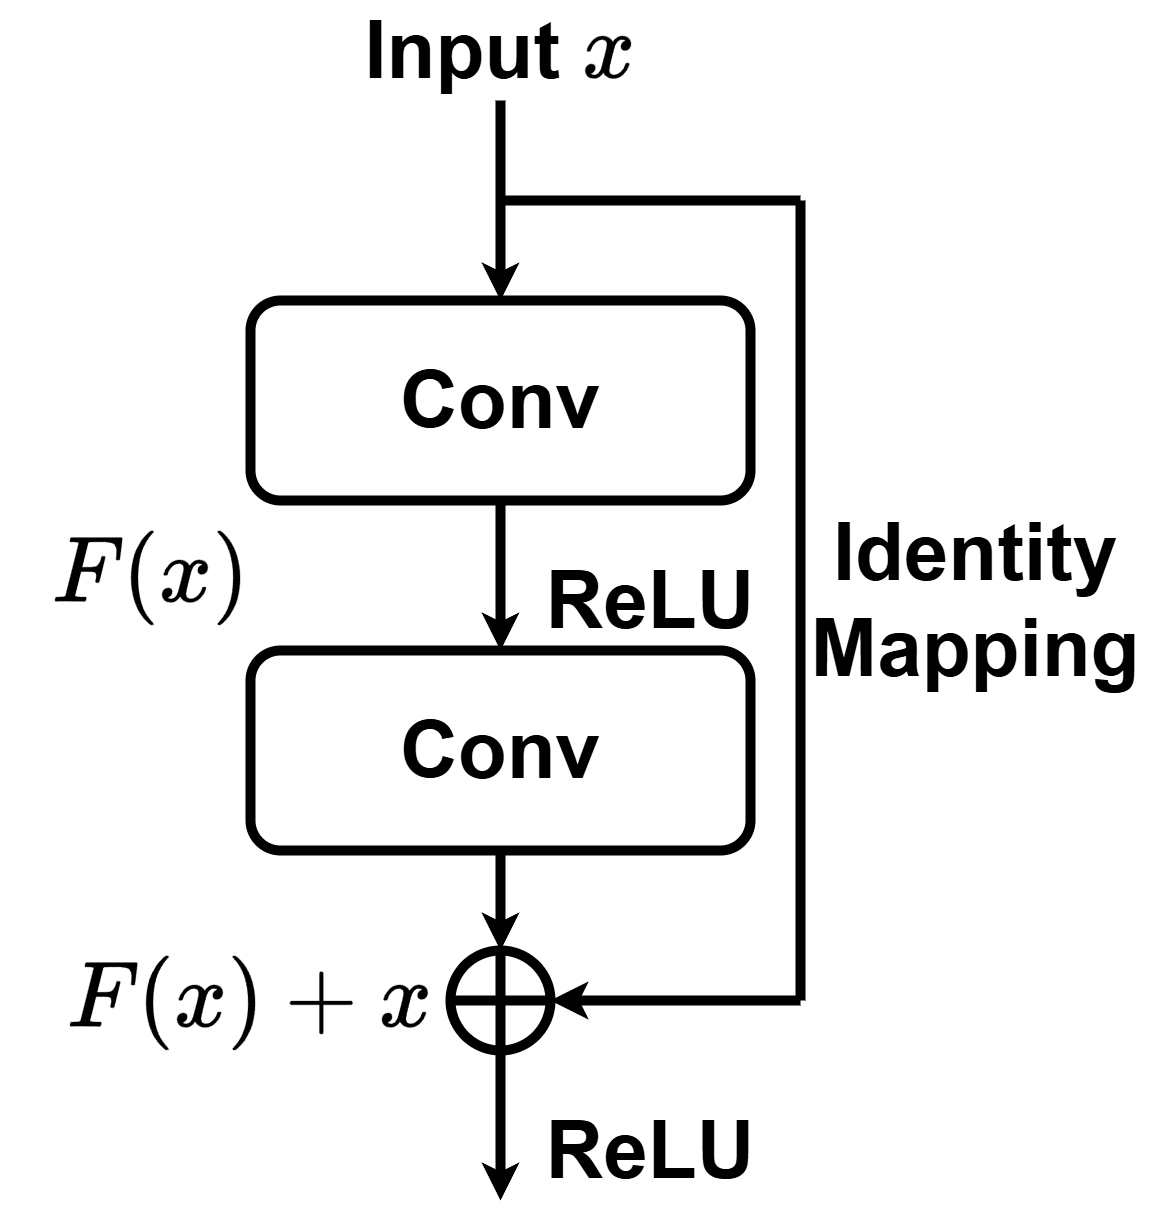
\includegraphics[width=0.8\linewidth]{figures/Fig1.png}
  \caption{Residual Learning}
  \label{fig:figure1}
\end{figure}
\subsection{Convolutional Neural Network}
A CNN typically comprises multiple convolutional layers, each consisting of several convolutional units. These layers leverage a backpropagation algorithm, such as gradient descent or its variants (e.g., conjugate gradient or AdaBoost), to optimise a chosen loss function. The core principle of convolution involves extracting progressively complex hierarchical features from the raw data. Initial convolutional layers focus on capturing low-level features, with subsequent layers progressively extracting more intricate representations. Compared to other network architectures, CNNs exploit sparse connectivity. This is achieved by utilizing kernels (weight matrices) that are smaller than the input data and enforcing local connectivity patterns between neurons in adjacent layers. This approach efficiently captures the complex interactions between units while simultaneously mitigating the risk of overfitting. Notably, each kernel is shared across the entire visual field during the convolution operation, requiring training only once. This eliminates the need to learn separate weight sets for each location, making CNNs highly efficient in applying the same linear transformation to local regions throughout the input data, effectively describing spatial transformations within the data.

The ReLU activation function is a popular choice for convolutional neural networks due to its ability to accelerate the training process. Mathematically, it is defined as:
\begin{equation}
    f(x) = max(0, x)
\end{equation}

CNNs frequently employ pooling layers, a form of downsampling. This technique is effective because the exact location of a feature is often less critical than its relative position within the data. Pooling progressively reduces the data dimensionality, leading to a corresponding decrease in the number of parameters and computational cost. This reduction also aids in mitigating overfitting. Furthermore, pooling operations introduce a degree of invariance to small translations of the input data within the extracted feature maps.  Max pooling, the most prevalent pooling technique, selects the maximum value from predefined regions (clusters) of neurons in the preceding layer.

Leveraging the remarkable capabilities of Convolutional Neural Networks (CNNs), researchers have extensively explored their application in near-infrared (NIR) spectroscopy analysis across a diverse range of problem domains. \cite{chakravartula2022use} used CNN combined with FT-NIR spectroscopy to predict food adulteration. This study combined CNN with Data augmentation (DA) with either autoscaling (AS) and/or standard normal variate (SNV) pre-treatment showed better prediction performances with RMSEP (0.76–0.82\%) and BIASP (-1.00 × $10^{-2}$  to -1.00 × $10^{-1}$\%) that were better to comparable to those of PLS and/or iPLS models (0.72 < \% RMSEP < 3.045; -7.98 × $10^{-2}$ < \% BIASP < 8.63 × $10^{-2}$) for the adulterants tested. Another study of \cite{hosseinpour2023cnn} developed 1D CNN models using absorbance spectral data to predict soil properties. This work confirms the potential of deep learning models combined with VIS–NIR spectral data to provide a rapid and non-destructive method for evaluating key soil properties.

\subsection{Kolmogorov-Arnold Network - A high-performing alternative to Multi-Layer Perceptrons}
The Kolmogorov-Arnold representation theorem, a cornerstone of approximation theory, establishes the capability of representing any continuous multivariate function on a bounded domain using a combination of simpler functions. This theorem states that such a function can be expressed as a finite composition of univariate functions and basic addition operations. Mathematically, for a continuous function $f: [0, 1]^{n_{in}} \rightarrow \mathbb{R}^{n_{out}}$, with $n_{in}$ and $n_{out}$ denote dimension of input and output, respectively, the theorem guarantees the existence of continuous univariate functions $\psi_q$ and $\phi_{p, q}$ such that:
\begin{equation}
    f(x) = \sum_{q=1}^{2n_{in} + 1} \psi_q(\sum_{p=1}^{n_{in}}\phi_{p, q}(x_p)) = 1
\end{equation}
Where $x = (x_1,...,x_{n_{in}})$, $\phi_{p, q}: [0, 1]\rightarrow \mathbb{R}$ and $\psi_q: \mathbb{R} \rightarrow \mathbb{R}$

Building upon the Kolmogorov-Arnold representation theorem, which guarantees any continuous multivariable function within a bounded domain can be expressed as a sum of single-variable continuous functions, \cite{liu2024kan} introduced Kolmogorov-Arnold Networks (KANs). These networks aim to capture both the compositional structure of the function (external degrees of freedom) and efficiently approximate the individual components (internal degrees of freedom). Within a KAN layer, \cite{liu2024kan} employed a combination of spline functions and SiLU activations with learnable coefficients. While splines excel at representing low-dimensional data, they suffer from the curse of dimensionality in higher dimensions due to the lack of inherent compositional structure. Conversely, Multi-Layer Perceptrons (MLPs) exhibit less sensitivity to the curse of dimensionality due to their feature learning capabilities. However, MLPs can be less accurate in low-dimensional settings due to their inefficiency in optimizing single-variable functions. Therefore, an ideal model for function approximation should effectively balance capturing the compositional nature of the function and efficiently approximating the underlying univariate components. A more in-depth explanation of KANs can be found in the work of \cite{liu2024kan}

A KAN consists of multiple stacked KAN layers. Each KAN layer processes $n_{in}$-dimensional input vectors and generates $n_{out}$-dimensional output vectors. Mathematically, a KAN layer can be represented as a matrix where each element corresponds to a 1D function:
\begin{equation}
    \Psi = \{\phi_{p, q}\}; p = 1, 2,\ldots, n_{in}; q = 1, 2,\ldots,n_{out} 
\end{equation}
Where the functions $\phi_{p, q}$ have learnable parameters.

The architecture of a KAN can be represented as a sequence of integers, denoted as $[n_0, n_1,..., n_L]$, where $n_l$ signifies the number of nodes (neurons) in the $l^{th}$ layer. Each neuron within a layer is identified using a two-part index $(l, i)$, where $l$ represents the layer number and $i$ represents the specific neuron within that layer. Furthermore, $x_{l, i}$ denotes the activation value of the $(l, i)$ neuron.

It's important to note that there exists $n_ln_{l+1}$ activation functions that connect consecutive layers $l$ and $l + 1$. Each activation function bridges the output of a specific neuron $(l, i)$ in layer $l$ with the input of another neuron $(l + 1, j)$ in the subsequent layer $(l + 1)$. The notation for this activation function connecting these two neurons is:
\begin{equation}
    \phi_{l, i, j}; l = 0,\ldots,L-1; i = 1,\ldots,n_l; j = 1,\ldots,n_{l+1}
\end{equation}

In contrast to MLPs where activation functions are applied to node outputs, KANs employ activation functions on the edges connecting neurons. This distinction is crucial. In a KAN layer, the pre-activation value denoted by $\phi_{l, i, j}$ is calculated using $x_{l, i}$, the activation value of the source neuron $(l, i)$. The activation function then transforms this pre-activation value into the post-activation value, denoted by $\tilde{x}_{l, i,j}$. Subsequently, the post-activation values from all incoming edges to a target neuron $(l + 1,j)$ are summed to determine its activation value, $x_{l+1,j}$:
\begin{equation}
    x_{l+1,j} = \sum_{i+1}^{n_l} \tilde{x}_{l,i,j} = \sum_{i+1}^{n_l} \phi_{l, i, j}(x_{l,i})
\end{equation}

This can be presented in a matrix form as follows:
\begin{equation}
    x_{l+1} = \begin{pmatrix} \phi_{l, 1, 1} & \cdots & \phi_{l, 1, n_l} \\
                              \vdots & \ddots & \vdots \\
                              \phi_{l, n_{l+1}, 1} & \cdots & \phi_{l, n_{l+1}, n_l}
    \end{pmatrix} x_l = \Psi_lx_l 
\end{equation}
Where $\Psi_l$ is the function matrix corresponding to the $l^{th}$ KAN layer. Then, a general KAN is expressed as a composition of $L$ layers:
\begin{equation}
    KAN(x) = (\Psi_{L-1} \circ \bold{\Psi}_{L-2} \circ \ldots \circ \bold{\Psi}_{1} \circ \bold{\Psi}_{0})
\end{equation}

\section{Methodology}\label{sec3}
\subsection{NirMACNet}\label{sec3.1}
NIR spectroscopy offers a promising approach for predicting substance concentrations through regression analysis. However, several challenges remain. Firstly, conventional CNN architectures utilize single-scale convolutional kernels, limiting feature extraction to a specific range. Real-world NIR spectra exhibit inherent variability due to factors like component changes, system variations, or sampling frequency fluctuations. Consequently, a fixed kernel size may not effectively capture features across diverse data scales. Secondly, NIR spectra acquisition often occurs under non-ideal conditions. To achieve optimal prediction accuracy, the model's ability to analyze data under varying operational circumstances becomes crucial.

To address the limitations of single-scale kernels, this paper introduces  NirMACNet, a novel deep learning architecture that leverages a multi-scale convolutional kernel approach. The fundamental building block of our model is a basic CNN block, which is constructed as follows:

\begin{equation}
\begin{split}
    y &= W \otimes x + b \\
    s &= BN(y) \\
    h &= ReLU(s) \\
\end{split}
\end{equation}

The convolution operation (denoted by $\otimes$) is employed within this block. Batch normalization (BN) is subsequently applied, enhancing the model's generalization capabilities and enabling the utilization of significantly higher learning rates.

Building upon the basic CNN block, the NirMACNet subblock is constructed by stacking two of these blocks sequentially, as illustrated in Figure \ref{fig:figure2}. As previously discussed, residual learning allows networks to achieve significant depth without encountering the degradation problem. Therefore, residual connections between each CNN subblock are incorporated to facilitate the construction of a deeper network capable of extracting intricate features. Denoting the basic CNN block as Basic, the subblock can be formally represented as follows:

\begin{equation}
    \begin{split}
    h_1 &= Basic(x) \\ 
    h_2 &= Basic(h_1) \\
    y &= h_2 + x \\
    \hat{h} &= ReLU(y) \\
    \end{split}
\end{equation}
\begin{figure}[!h]
  \centering
  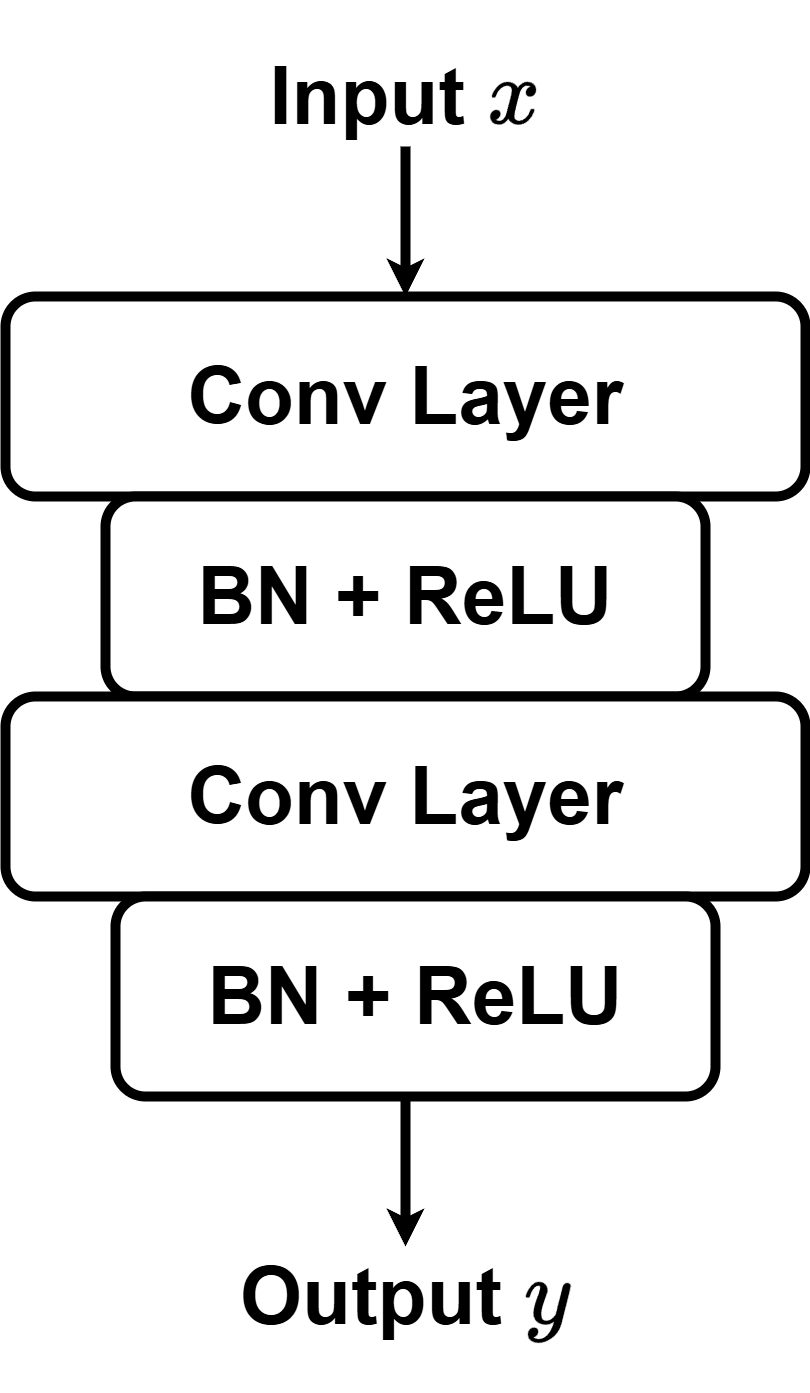
\includegraphics[width=0.4\linewidth, angle=90]{figures/Fig2.png}
  \caption{NirMACNet subblock}
  \label{fig:figure2}
\end{figure}

By stacking multiple subblocks sequentially, a complete CNN block can be constructed as depicted in Figure \ref{fig:figure3}. Denoting the subblock as Subblock, the formal representation of the CNN block becomes:
\begin{equation}
    \begin{split}
        \hat{h}_1 &= subblock(x) \\
        \hat{h}_2 &= subblock(\hat{h}_1) \\ 
        \hat{h}_3 &= subblock(\hat{h}_2) \\
    \end{split}
\end{equation}
\begin{figure}[!h]
  \centering
  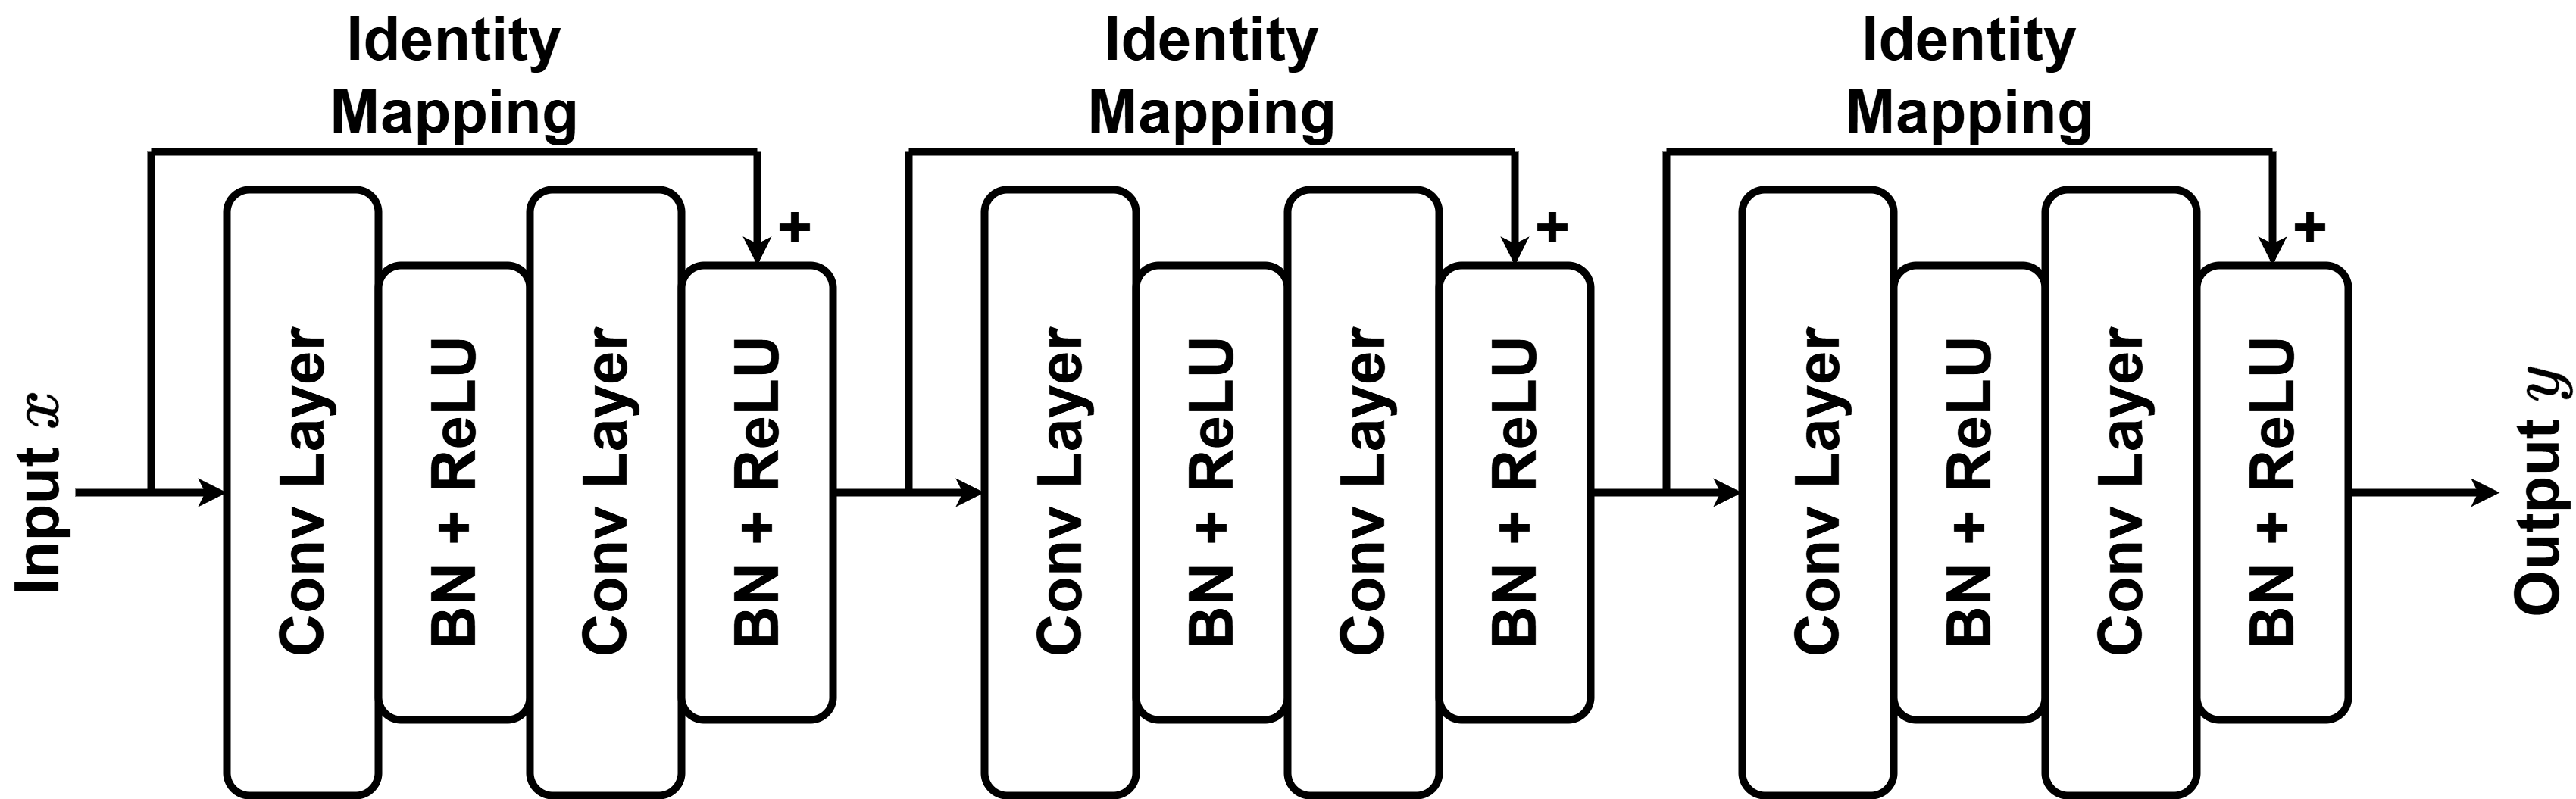
\includegraphics[width=0.9\linewidth]{figures/Fig3.png}
  \caption{Complete CNN Block for NirMACNet}
  \label{fig:figure3}
\end{figure}

Unlike conventional approaches that rely on downsampling or averaging the original data, our proposed method leverages multi-scale convolutional kernels. Downsampling and averaging techniques primarily reduce data dimensionality but may not effectively capture underlying feature variations. In contrast, employing kernels of varying sizes empowers CNN to extract features from the original data across multiple scales and from diverse perspectives. This enables the model to learn a more comprehensive representation of the underlying data structure.

Figure \ref{fig:figure4} presents a graphical illustration of the proposed NirMACNet architecture. NIR spectra data serves as the direct input for the model. Leveraging the strength of CNNs in feature extraction, we construct a network with three consecutive CNN blocks. Each block employs convolutional kernels of different sizes to capture features from varying receptive fields. Specifically, the kernel sizes across the blocks are $1\times3$, $1\times5$, and $1\times7$. This design choice stems from the observation that feature maps obtained using larger kernels can be equivalently extracted through multiple layers with smaller kernels. However, larger kernels inherently increase model complexity and computational cost. Therefore, smaller kernels are generally preferred in practice.

\begin{figure}[!h]
  \centering
  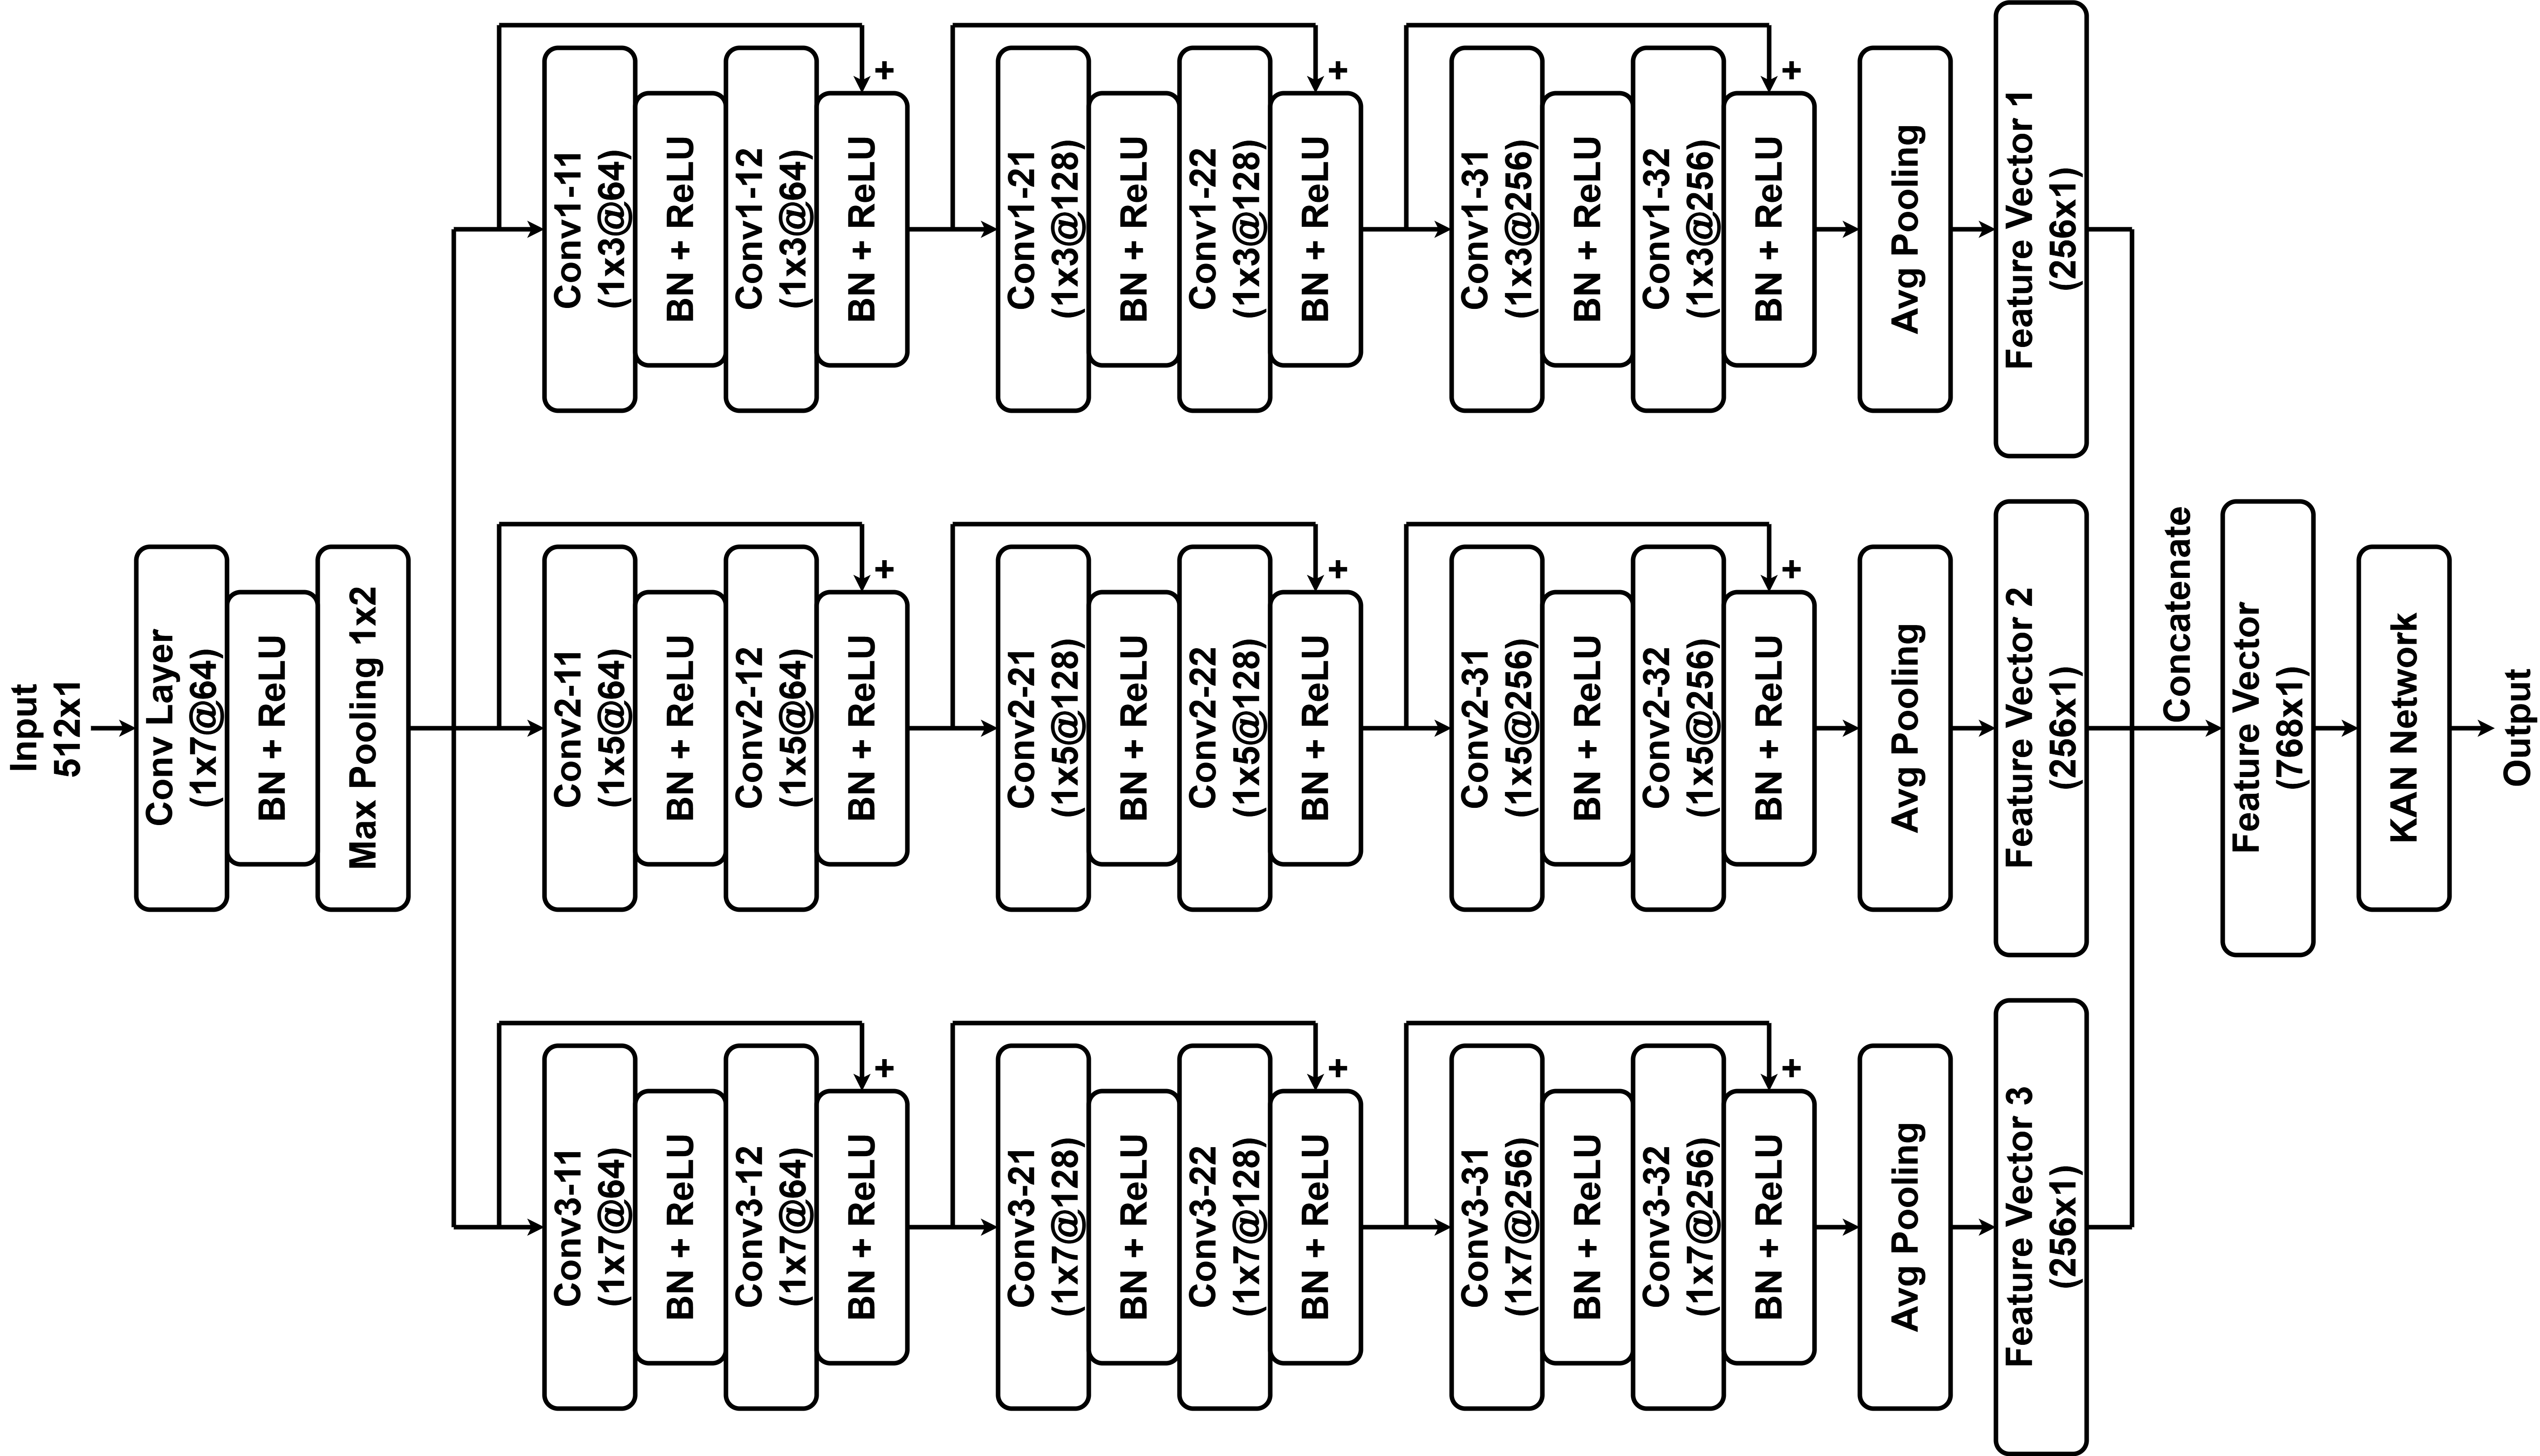
\includegraphics[width=0.9\linewidth]{figures/Fig4.png}
  \caption{NirMACNet Architecture}
  \label{fig:figure4}
\end{figure}

Unlike traditional CNN models, the pooling operation within each CNN block is omitted to preserve detailed features. Following the convolution blocks, the extracted features are fed into a global average pooling layer. This layer enhances the model's robustness against input translations, reduces the number of trainable weights, and mitigates overfitting. Average pooling was opted to retain the global feature maps extracted by the convolutional layers. Subsequently, the feature vectors obtained from the pooling layers in each block are concatenated into a single vector. This vector then serves as the input for a fully connected network, followed by a KAN for regression analysis. The KAN network is configured with an input layer of 768 dimensions, followed by four hidden layers with decreasing dimensionality (256, 128, 64, 32), and concludes with a single output unit.

\section{Experimental results} \label{sec:e}
\subsection{Dataset}
To assess the generalizability and practical applicability of the proposed model, two spectroscopic datasets from distinct domains are utilized in this study: a soil spectral dataset \cite{meszaros2025vis} derived from a national monitoring system, and a milk spectral dataset \cite{diaz2023near} collected from a controlled experimental farm. These datasets represent different material types and measurement conditions, thereby enabling a comprehensive evaluation of the model’s robustness across diverse real-world scenarios.
\subsubsection{Soil Spectral Dataset}
A newly compiled Vis-NIR soil spectral dataset \cite{meszaros2025vis} is derived from the Hungarian Soil Degradation Observation System. The dataset comprises 5,490 high-resolution soil reflectance spectra (350–2,500 nm), combined with comprehensive laboratory reference data on soil physicochemical properties. Each spectrum represents a composite soil sample collected from one of 2,030 parcels across 294 representatively selected Hungarian agricultural farms, ensuring national coverage and geographic diversity.

Each measurement includes five repeated reflectance spectra, averaged for a single representative spectrum per sample. These spectra were recorded under laboratory conditions with a contact probe setup, following rigorous calibration procedures using a Spectralon white reference panel. Spectral preprocessing included splice correction and the removal of noisy measurements based on the standard deviation of repeated scans. Final spectra were interpolated to 1 nm resolution, resulting in 2,151 wavelength variables per sample. Figure \ref{fig:figure6} presents the spectral measurements of the Soil Spectral Dataset.

\begin{figure}[!h]
  \centering
  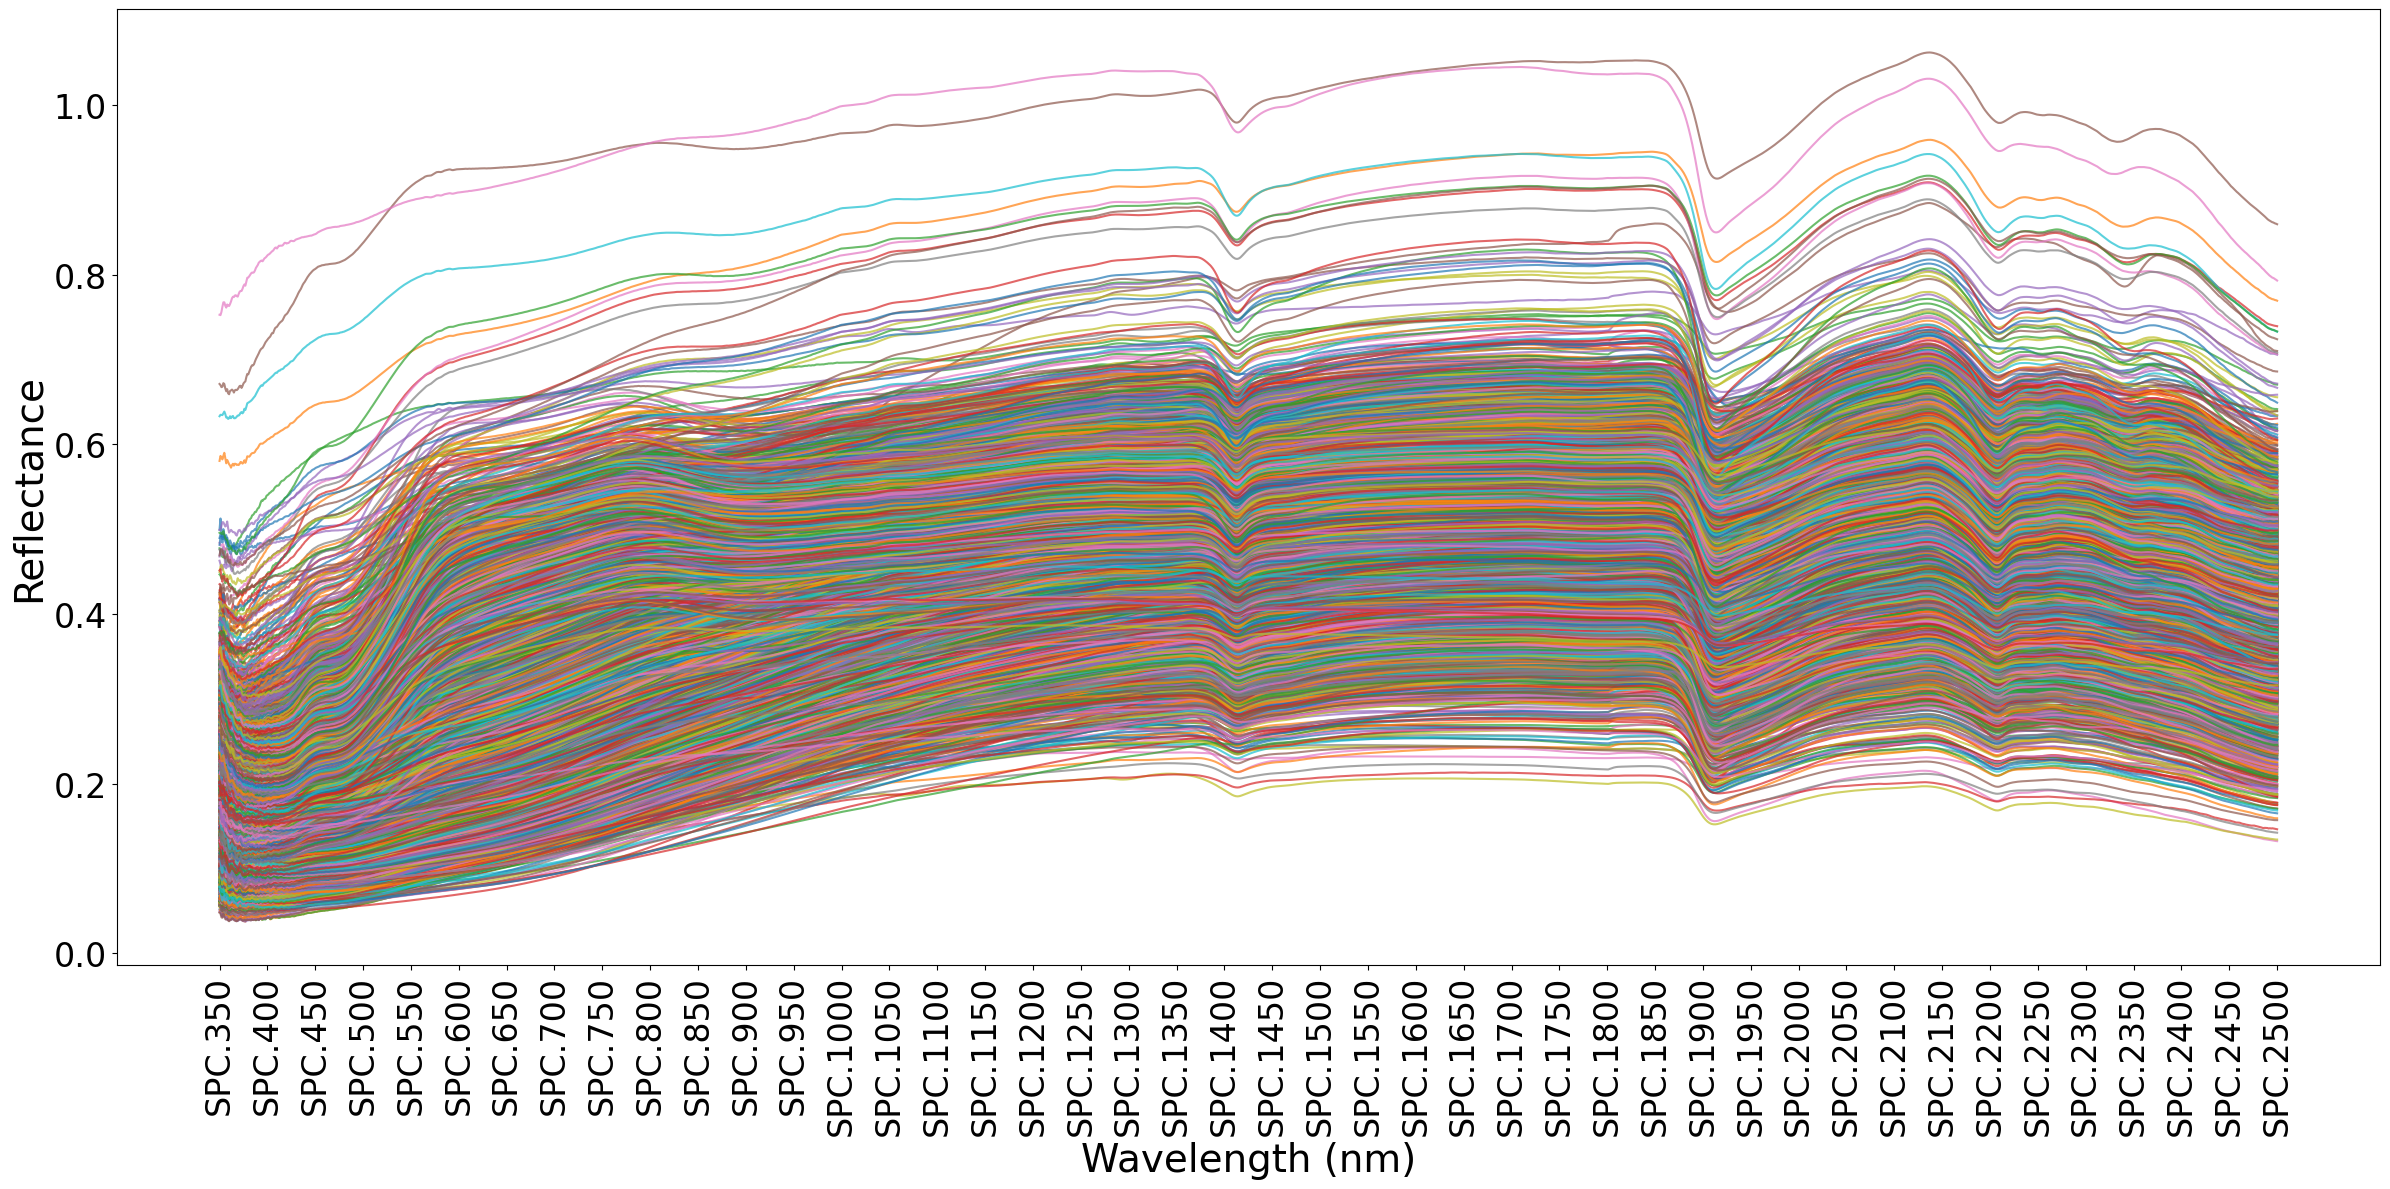
\includegraphics[width=\linewidth]{figures/Fig6.png}
  \caption{Vis–NIR Spectral Reflectance of the Soil Spectral Dataset}
  \label{fig:figure6}
\end{figure}


Corresponding soil reference properties include both chemical and physical attributes: pH (KCl), soil organic matter (SOM), calcium carbonate \( (\text{CaCO}_3) \), total salt content (TSC), total nitrogen (TN), available phosphorus \( (\text{P}_2\text{O}_5) \), available potassium \( (\text{K}_2\text{O}) \), available potassium \((\text{K}_2\text{O})\), and plasticity index (PLI). Table \ref{tab:table6} presents a summary of the chemical and physical attributes in the soil spectral dataset.

\begin{table*}[!h]
\centering
\begin{tabular}{ccccccccc}
\hline
& pH\_KCl & PLI & SOM & \(\text{CaCO}_3\) & TSC & TN & \(\text{P}_2\text{O}_5\) & \(\text{K}_2\text{O}\) \\
\hline
Mean & 7.36 & 42.68 & 1.63 & 7.81 & 0.04 & 12.36 & 162.69 & 197.12 \\
Std & 0.85 & 9.03 & 0.99 & 10.16 & 0.04 & 16.32 & 297.26 & 160.74 \\
\hline
\end{tabular}
\caption{Summary of Chemical and Physical Attributes in the Soil Spectral Dataset}\label{tab:table6}
\end{table*}

The original soil spectral data, consisting of 2,150 wavelength variables, are utilized as direct input to the model. However, to align with the architectural requirements of the model, which is optimized for input dimensions that are powers of two, the spectral dimensionality is reduced to 2,048. This adjustment is accomplished through a combination of spectral truncation and dimensionality selection. This preprocessing step ensures compatibility with the model’s structural constraints and facilitates efficient data processing.

\subsubsection{Milk Spectral Dataset}
A milk spectral dataset, utilized in this study, is compiled by \cite{diaz2023near}. This dataset encompasses 1224 NIR spectral measurements of raw milk samples collected over eight weeks at the Hooibeekhoeve experimental farm (Geel, Belgium). These spectra are provided in transmittance mode, covering a wavelength range of 960–1690 nm with a resolution of 2.86 nm/pixel, resulting in a total of 256 wavelengths. Each measurement incorporates three components:
\begin{itemize}
    \item Raw milk sample: Spectral measurement of the raw milk itself
    \item White spectral reference: Spectrum of a white reference material for baseline correction
    \item Dark spectral reference: Spectrum acquired with no light source for background noise removal
\end{itemize}
All measurements employed an integration time of 100 ms and averaged 100 individual spectra for improved signal quality. Additionally, the dataset includes corresponding laboratory reference values for the three primary components of raw milk (fat, protein, and lactose), along with urea and somatic cell count (SCC). Importantly, each data point represents a unique milk sample, with all samples originating from 41 cows.

Table \ref{tab:table1} summarises the reference values for the five milk compounds analyzed (fat, protein, lactose, urea, and somatic cell count). Figure \ref{fig:figure5} presents the spectral measurements. The left side of the figure depicts the raw transmitted spectra, displayed in digital counts. The right side shows the normalized transmittance spectra. 

\begin{table*}[!h]
\centering
\begin{tabular}{cccccccccccc}
\hline
\multirow{2}{*}{Week} & \multirow{2}{*}{N} & \multicolumn{2}{c}{Fat} & \multicolumn{2}{c}{Protein} & \multicolumn{2}{c}{Lactose} & \multicolumn{2}{c}{Urea} & \multicolumn{2}{c}{SCC} \\ \cline{3-12} 
  &  & Mean & Std & Mean & Std & Mean & Std & Mean & Std & Mean & Std \\ \hline
1 & 348 & 3.45 & 0.85 & 3.45 & 0.34 & 4.74 & 0.15 & 29.92 & 5.83 & 172.90 & 400.54 \\ 
2 & 190 & 3.45 & 0.80 & 3.42 & 0.33 & 4.72 & 0.14 & 30.08 & 5.05 & 132.25 & 249.71 \\ 
3 & 79 & 3.50 & 0.90 & 3.44 & 0.36 & 4.70 & 0.16 & 28.04 & 4.48 & 139.91 & 300.26 \\ 
4 & 60 & 3.34 & 0.76 & 3.40 & 0.34 & 4.70 & 0.17 & 25.10 & 5.66 & 130.03 & 204.82 \\ 
5 & 167 & 3.47 & 0.72 & 3.47 & 0.33 & 4.67 & 0.15 & 28.07 & 4.04 & 227.13 & 503.50 \\ 
6 & 96 & 3.58 & 0.86 & 3.41 & 0.32 & 4.69 & 0.14 & 25.50 & 4.30 & 237.30 & 500.77 \\ 
7 & 168 & 3.66 & 0.72 & 3.36 & 0.32 & 4.67 & 0.17 & 22.99 & 3.60 & 191.02 & 362.29 \\ 
8 & 162 & 3.72 & 0.83 & 3.39 & 0.34 & 4.67 & 0.18 & 26.30 & 4.07 & 187.75 & 255.78 \\ 
\hline
\end{tabular}
\caption{Summary of milk composition}\label{tab:table1}
\end{table*}

\begin{figure}[!h]
  \centering
  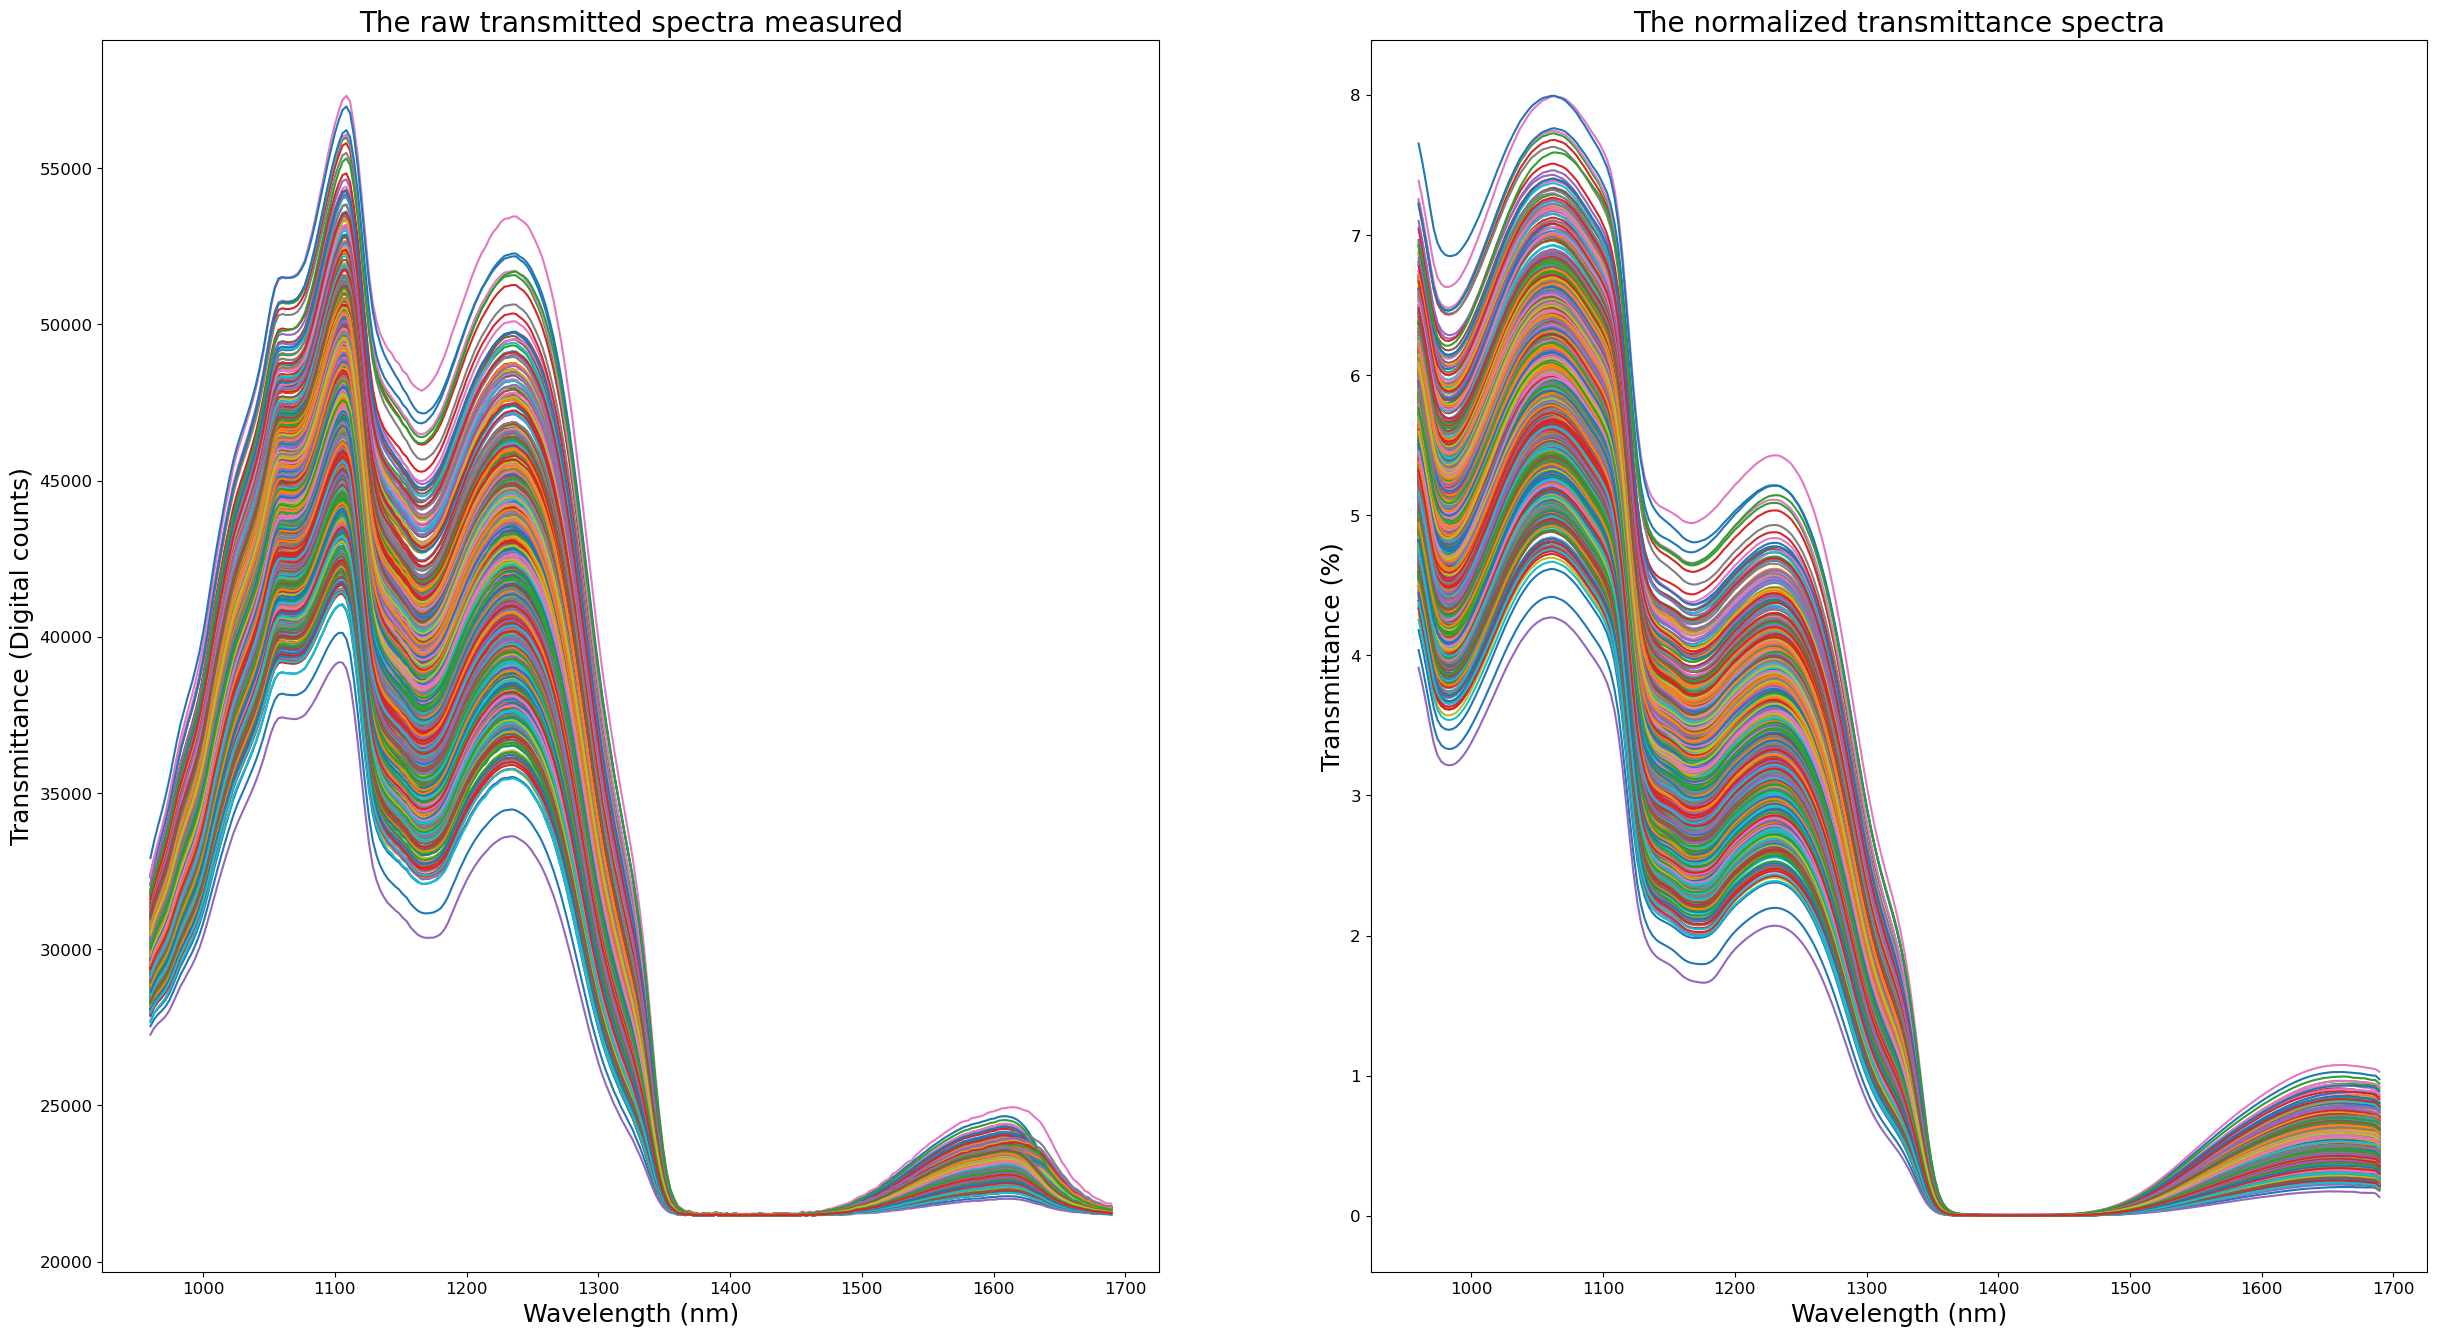
\includegraphics[width=\linewidth]{figures/Fig5.png}
  \caption{Raw Transmitted Spectra (left) and Normalized Transmittance Spectra (right) of the Milk Dataset}
  \label{fig:figure5}
\end{figure}

\subsection{Experimental results} 
\subsubsection{Implementation details}	
The entire training and evaluation process was conducted on the Windows 10 operating system, utilizing an Intel® Xeon® Platinum 8470Q processor and an NVIDIA DGX A100 graphics card. The software employed Python version 3.10 and the Pytorch CUDA 12.1 framework. 
\subsubsection{Training details}
The entire dataset is divided into 5 non-overlapping subsets. With each subset, that subset is used as the testing set, and the rest are used as the training set. The evaluation results of the model are averaged after 5 evaluations.

In this work, models underwent training for 200 epochs, leveraging SGD as the optimizer with a starting learning rate of 1e-5. The learning rate was scheduled using the Cosine Annealing with Warm-Up Learning Rate method. Mean Squared Error (MSE) served as the loss function during training.

The performance of NirMACNet is compared with traditional models such as SVR, ENET, Random Forest, PLS, and XGBoost, as well as several advanced deep learning models, including the Vanilla Transformer \cite{vaswani2017attention}, LSTM \cite{graves2012long}, and CNN-LSTM \cite{khorram2023hybrid}. Hyperparameter tuning was performed to determine optimal hyperparameter sets for these traditional models using the Gridsearch method \cite{liashchynskyi2019grid}; the optimal hyperparameters are shown in Table \ref{tab:table3}.

\renewcommand{\arraystretch}{1.5}
\setlength{\tabcolsep}{4pt}
\begin{table}
    \centering
    \begin{tabular}{ccccc}
        \hline
        \textbf{Algorithm} & \textbf{Parameters} & \textbf{Minimum} & \textbf{Maximum} & \textbf{Optimal} \\
        \hline
        SVR & cost (C) & $9.77 \times 10^{-4}$ & 32 & 0.01 \\
                     & margin (epsilon) & 0 & 0.2 & 0.05\\
        \hline
        ENET & penalty & $10^{-10}$ & 1 & 0.62 \\
             & mixture (alpha) & 0.05 & 1 & 0.7 \\
        \hline
        PLS & predictor\_prop & 0 & 1 & 0.6 \\
            & num\_comp & 1 & 4 & 3 \\
        \hline
        Random Forest & tree\_depth & 1 & 15 & 12 \\
                      & n\_trees & 1 & 2000 & 1850 \\
                      & min\_rows & 1 & 40 & 32 \\
        \hline 
        XGBoost & tree\_depth & 1 & 15 & 12 \\
                & n\_trees & 1 & 2000 & 1800 \\
                & learn\_rate (eta) & 0.001 & 0.4 & 0.05 \\
                & early\_stop & 3 & 20 & 5 \\
        \hline 
    \end{tabular}
    \caption{Ranges of hyperparameters used in tuning of best results for various machine learning techniques}
    \label{tab:table3}
\end{table}

\subsubsection{Evaluate Metrics}
The evaluation was conducted using 2 metrics: Mean Square Error (MSE) and R-squared ($R^2$)

MSE measures the mean error of predicted values $\hat{y}_i$, in comparison to actual values $y_i$ in the test dataset with $n$ data samples. The MSE calculation is delineated by the formula:
\begin{equation}
    MSE = \frac{1}{n} \sum_{i=1}^{n} (y_i - \hat{y}_i)^2
\end{equation}

$R^2$, also known as the coefficient of determination, serves to evaluate the congruence between a model and the data. The $R^2$ value spans a range from 0 to 1, with:
\begin{itemize}
    \item $R^2 = 0$: indicating that the model does not explain any variation in the data and is entirely uncorrelated to it;
    \item $R^2 = 1$: indicating that the model completely explains all the variations in the data and perfectly fits the data;
    \item $R^2 \in (0, 1)$: signifying the relative degree of fit of the model to the data; the higher the $R^2$ value, the better the model is at explaining variations in the data.
\end{itemize}

Given $y_i$ as the actual value, $\hat{y}_i$ as the predicted value, and $\bar{y}$ representing the mean value of the target variable, the $R^2$ value is calculated using the following formula:
\begin{equation}
    R^2 = 1 - \frac{\sum_{i=1}^{n} (y_i - \hat{y}_i)^2}{\sum_{i=1}^{n} (y_i - \bar{y}_i)^2}
\end{equation}

\subsubsection{Evaluation an Discussion}
\textbf{Comparative Analysis}: On the high-dimensional Soil Spectral Dataset, comprising 2048 input features, as can be seen from Table \ref{tab:table7}, NirMACNet consistently surpasses all baseline models across the eight soil property prediction tasks. It achieves the lowest MSE and the highest R2-score in all cases, reflecting superior predictive accuracy and generalization capability. Meanwhile, deep learning architectures such as LSTM, CNN-LSTM, and Transformer exhibit notable improvements over traditional machine learning approaches (SVR, ENET, PLS). Notably, Vanilla Transformer's performance is constrained by overfitting, primarily due to the disproportion between its number of parameters and the relatively limited number of training samples (Table \ref{tab:table6}). In contrast, NirMACNet demonstrates strong resilience to overfitting, which can be attributed to its tailored architectural design optimized for capturing complex spectral representations. These findings underscore NirMACNet’s effectiveness in modeling intricate patterns inherent in high-dimensional spectral data.

\begin{table*}[!h]
\centering
\resizebox{\textwidth}{!}{%
\begin{tabular}{ccccccccc}
\hline
\textbf{Model} & \textbf{pH\_KCl} & \textbf{PLI} & \textbf{SOM} & \textbf{CaCO$_3$} & \textbf{TSC} & \textbf{TN} & \textbf{P$_2$O$_5$} & \textbf{K$_2$O} \\
\hline
\multicolumn{9}{c}{\textit{MSE}} \\
\hline
SVR           & 0.201 & 8.034   & 0.794  & 40.218   & 0.002  & 89.683   & 159.842  & 79.942  \\
ENET          & 0.246 & 9.478   & 0.911  & 48.396   & 0.003  & 100.291  & 180.325  & 90.081  \\
PLS           & 0.282 & 10.243  & 0.939  & 52.114   & 0.003  & 109.774  & 190.673  & 94.893  \\
Random Forest & 0.139 & 6.513   & 0.647  & 29.806   & 0.002  & 70.532   & 120.184  & 60.127  \\
XGBoost       & 0.118 & 5.927   & 0.604  & 25.017   & 0.002  & 60.438   & 105.492  & 49.713  \\
Transformer   & 0.076 & 4.179   & 0.448  & 17.856   & 0.001  & 42.316   & 80.217   & 35.198  \\
LSTM          & 0.063 & 3.496   & 0.358  & 14.972   & 0.001  & 35.104   & 65.284   & 28.107  \\
CNN-LSTM      & 0.049 & 3.217   & 0.321  & 13.471   & 0.001  & 32.208   & 59.946   & 25.948  \\
NirMACNet     & \textbf{0.045} & \textbf{2.931} & \textbf{0.283} & \textbf{12.083} & \textbf{0.001} & \textbf{29.962} & \textbf{54893} & \textbf{24136} \\
\hline
\multicolumn{9}{c}{\textit{R2-score}} \\
\hline
SVR           & 0.603 & 0.624   & 0.479  & 0.454    & 0.596  & 0.501   & 0.523   & 0.578  \\
ENET          & 0.549 & 0.579   & 0.426  & 0.378    & 0.551  & 0.456   & 0.454   & 0.542  \\
PLS           & 0.516 & 0.564   & 0.411  & 0.352    & 0.519  & 0.404   & 0.419   & 0.517  \\
Random Forest & 0.713 & 0.719   & 0.596  & 0.577    & 0.682  & 0.604   & 0.636   & 0.665  \\
XGBoost       & 0.752 & 0.754   & 0.634  & 0.627    & 0.718  & 0.659   & 0.692   & 0.722  \\
Transformer   & 0.846 & 0.817   & 0.729  & 0.718    & 0.801  & 0.741   & 0.764   & 0.799  \\
LSTM          & 0.901 & 0.875   & 0.797  & 0.761    & 0.858  & 0.786   & 0.809   & 0.846  \\
CNN-LSTM      & 0.914 & 0.891   & 0.818  & 0.776    & 0.881  & 0.814   & 0.827   & 0.864  \\
NirMACNet     & \textbf{0.927} & \textbf{0.909} & \textbf{0.843} & \textbf{0.803} & \textbf{0.894} & \textbf{0.832} & \textbf{0.853} & \textbf{0.879} \\
\hline
\end{tabular}%
}
\caption{Evaluating performance of NirMACNet compared to other models using MSE $(\downarrow)$ and R2-score $(\uparrow)$ on the Soil Spectral Dataset}\label{tab:table7}
\end{table*}

On the Milk Spectral Dataset, characterized by a lower input dimensionality (256 features), Table \ref{tab:table5} shows that NirMACNet again achieves the highest predictive performance across all five milk quality indicators: Fat, Protein, Lactose, SCC, and Urea. It attains the lowest MSE and the highest R2 scores, marginally outperforming other deep learning models such as CNN-LSTM and LSTM. Traditional machine learning models perform comparatively poorly, likely due to their limited capacity to capture nuanced relationships in spectral data. Although the Transformer model demonstrates competitive results, it tends to exhibit signs of overfitting in this small-sample context, a pattern also observed in the Soil Spectral Dataset. NirMACNet’s consistent superiority across both high- and low-dimensional spectral settings highlights its robustness and adaptability to varying data regimes.

\begin{table*}[!h]
\centering
\begin{tabular}{ccccc}
\hline
\textbf{Model} & LSTM & CNN-LSTM & Vanilla Transformer & NirMACNet \\
\hline
\textbf{Params} & 1.27M & 1.77M & 2.41M & 2.37M\\
\hline
\end{tabular}
\caption{Comparison of Model Parameter Counts Between NirMACNet and Other Deep Learning Architectures}\label{tab:table8}
\end{table*}

Although NirMACNet has a comparable number of parameters (2.37M) to the Vanilla Transformer (2.41M), as shown in Table \ref{tab:table8}, its architectural design offers a crucial advantage in terms of generalization and resistance to overfitting. Unlike sequential models such as LSTM (1.27M) and CNN-LSTM (1.77M), and even the Transformer, which relies heavily on stacked attention layers, NirMACNet leverages a parallel processing structure that enables it to extract diverse and complementary features simultaneously.

This parallelism reduces dependency on deep sequential processing and mitigates the risk of overfitting that often arises from overly complex or redundant parameterization. Each parallel module in NirMACNet can focus on different aspects of the input, allowing for richer feature representations. Therefore, despite having a similar parameter count to the Transformer, NirMACNet achieves a more efficient trade-off between model capacity and generalization performance. This makes it particularly well-suited for tasks with limited data or high variability, where robustness and the ability to generalize are critical.

In comparative analysis across both datasets, traditional machine learning methods are markedly less effective in handling high-dimensional spectral inputs, leading to suboptimal predictive performance. Deep learning models offer improvements but remain vulnerable to overfitting, especially in data-scarce scenarios. NirMACNet distinguishes itself by consistently delivering state-of-the-art results, owing to its architecture specifically designed for spectral regression tasks. Its demonstrated capacity to generalize across datasets with differing dimensionality and sample sizes affirms its potential as a robust and scalable solution for spectral-based prediction problems in both agricultural and food quality assessment domains.

\begin{table*}[!h]
\centering
\begin{tabular}{ccc@{\hspace{10pt}}c@{\hspace{10pt}}c@{\hspace{10pt}}c@{\hspace{10pt}}c}
\hline
\textbf{Model} & \textbf{Metric} & \textbf{Fat} & \textbf{Protein} & \textbf{Lactose} & \textbf{SCC} & \textbf{Urea} \\
\hline
\multirow{2}{*}{SVR} & MSE     & 0.503 & 0.219 & 0.297 & 159.874 & 65.137 \\
& R2-score      & 0.618 & 0.732 & 0.698 & 0.747   & 0.671 \\
\multirow{2}{*}{ENET} & MSE    & 0.552 & 0.263 & 0.339 & 169.912 & 70.084 \\
& R2-score     & 0.577 & 0.702 & 0.683 & 0.709   & 0.638 \\
\multirow{2}{*}{PLS} & MSE     & 0.597 & 0.254 & 0.351 & 174.783 & 72.045 \\
& R2-score      & 0.553 & 0.714 & 0.669 & 0.698   & 0.622 \\
Random & MSE & 0.403 & 0.198 & 0.284 & 149.926 & 60.098 \\
Forest & R2-score  & 0.701 & 0.758 & 0.722 & 0.779   & 0.688 \\
\multirow{2}{*}{XGBoost} & MSE & 0.349 & 0.181 & 0.247 & 145.062 & 58.037 \\
& R2-score  & 0.743 & 0.782 & 0.754 & 0.802   & 0.712 \\
Vanilla & MSE & 0.026 & 0.071 & 0.036 & 144.987 & 10.142 \\
Transformer & R2-score  & 0.891 & 0.899 & 0.851 & 0.859   & 0.848 \\
\multirow{2}{*}{LSTM} & MSE         & 0.004 & 0.036 & 0.018 & 136.983 & 5.012 \\
& R2-score & 0.992 & 0.964 & 0.911 & 0.950   & 0.939 \\
\multirow{2}{*}{CNN-LSTM} & MSE     & 0.003 & 0.032 & 0.017 & 135.897 & 4.943 \\
& R2-score & 0.994 & 0.966 & 0.913 & 0.951   & 0.944 \\
\multirow{2}{*}{NirMACNet} & MSE & \textbf{0.002} & \textbf{0.032} & \textbf{0.016} & \textbf{135.939} & \textbf{4.926} \\ 
& R2-score & \textbf{0.995} & \textbf{0.968} & \textbf{0.913} & \textbf{0.952} & \textbf{0.945} \\
\hline
\end{tabular}
\caption{Evaluating performance of NirMACNet compared to other models using MSE $(\downarrow)$ and R2-score $(\uparrow)$ on the Milk Spectral Dataset}\label{tab:table5}
\end{table*}


\textbf{Ablation Study}: The Multi-scale model is compared to its One-scale variants, and the replacement of MLP with KAN is also evaluated in this experiment. As can be seen from Table \ref{tab:table2}, the Multi-scale model using KAN as Regressor outperforms other models in predicting the concentration of all substances, achieving MSE values of 0.002, 0.032, 0.016, 135.939, and 4.926, and R2-score values of 0.995, 0.968, 0.913, 0.952, and 0.945 for Fat, Protein, Lactose, SCC, and Urea, respectively. In addition, replacing MLP with KAN shows a significant improvement of about 0.03 in R2-score, not only for the Multi-scale model but also for the One-scale model.

\begin{table*}[h]
\centering
\resizebox{0.9\textwidth}{!}{%
\begin{tabular}{c@{\hspace{10pt}}c@{\hspace{10pt}}c@{\hspace{10pt}}c@{\hspace{10pt}}c@{\hspace{10pt}}c}
\hline
\textbf{Model} & \textbf{Fat} & \textbf{Protein} & \textbf{Lactose} & \textbf{SCC} & \textbf{Urea} \\ 
\hline
\multicolumn{6}{c}{\textit{Regressor Type: MLP}} \\
\hline
\makecell{One-scale\\$1 \times 3$} & 0.004/0.993 & 0.061/0.921 & 0.020/0.909 & 138.625/0.937 & 8.682/0.926 \\ 
\makecell{One-scale\\$1 \times 5$} & 0.005/0.992 & 0.055/0.939 & 0.019/0.910 & 138.218/0.937 & 7.982/0.932 \\ 
\makecell{One-scale\\$1\times 7$} & 0.004/0.993 & 0.054/0.938 & 0.019/0.911 & 138.921/0.937 & 9.246/0.918 \\ 
\makecell{Multi\\scale} & 0.004/0.993 & 0.041/0.949 & 0.019/0.911 & 137.531/0.938 & 5.276/0.939 \\ 
\hline
\multicolumn{6}{c}{\textit{Regressor Type: KAN}} \\
\hline
\makecell{One-scale\\$1 \times 3$} & 0.003/0.994 & 0.052/0.940 & 0.018/0.910 & 137.339/0.945 & 5.911/0.938 \\ 
\makecell{One-scale\\$1 \times 5$} & 0.003/0.994 & 0.044/0.945 & 0.016/0.913 & 137.246/0.946 & 5.939/0.935 \\ 
\makecell{One-scale\\$1\times 7$} & 0.002/0.994 & 0.046/0.942 & 0.017/0.913 & 136.632/0.949 & 5.918/0.936 \\ 
\makecell{Multi\\scale} & \textbf{0.002}/\textbf{0.995} & \textbf{0.032}/\textbf{0.968} & \textbf{0.016}/\textbf{0.913} & \textbf{135.939}/\textbf{0.952} & \textbf{4.926}/\textbf{0.945} \\ 
\hline
\end{tabular}}
\caption{Evaluating One-scale and Multi-scale model performance using MSE \((\downarrow)\) and R2-score \((\uparrow)\)}\label{tab:table2}
\end{table*}

Tables \ref{tab:table4} highlight the impact of feature extraction on MLP and KAN models. While these models can learn directly from raw data and make predictions (features are implicitly learned during training), they might miss underlying patterns crucial for accurate predictions. This is because raw data may not directly represent the most important factors affecting the target variable. The inclusion of the feature extraction module proposed in this study addresses this limitation. By transforming the raw data into more informative features, the models can capture these hidden patterns more effectively. This significantly improves the model's performance, as evidenced by an increase of about 0.2 in R2-score for all prediction targets. In simpler terms, the extracted features provide a more refined view of the data, allowing the models to make more accurate predictions.

\begin{table*}[!h]
\centering
\resizebox{0.9\textwidth}{!}{%
\begin{tabular}{cc@{\hspace{10pt}}c@{\hspace{10pt}}c@{\hspace{10pt}}c@{\hspace{10pt}}c}
\hline
\textbf{Model} & \textbf{Fat} & \textbf{Protein} & \textbf{Lactose} & \textbf{SCC} & \textbf{Urea} \\ 
\hline
\multirow{2}{*}{MLP} & \multirow{2}{*}{0.878/0.570} & \multirow{2}{*}{0.319/0.712} & \multirow{2}{*}{0.410/0.688} & \multirow{2}{*}{188.157/0.663} & \multirow{2}{*}{74.180/0.602} \\ 
& & & & & \\
\multirow{2}{*}{KAN} & \multirow{2}{*}{0.645/0.613} & \multirow{2}{*}{0.213/0.754} & \multirow{2}{*}{0.326/0.692} & \multirow{2}{*}{185.276/0.702} & \multirow{2}{*}{68.942/0.663} \\ 
& & & & & \\
\makecell{Multi-scale\\MLP} & 0.004/0.993 & 0.041/0.949 & 0.019/0.911 & 137.531/0.938 & 5.276/0.939 \\ 
\makecell{Multi-scale\\KAN} & \textbf{0.002}/\textbf{0.995} & \textbf{0.032}/\textbf{0.968} & \textbf{0.016}/\textbf{0.913} & \textbf{135.939}/\textbf{0.952} & \textbf{4.926}/\textbf{0.945} \\ 
\hline
\end{tabular}}
\caption{Evaluating performance of MLP and KAN with/without Feature Extractor using MSE $(\downarrow)$ and R2-score $(\uparrow)$}\label{tab:table4}
\end{table*}

\textbf{Discussion}: We employ SHAP (SHapley Additive exPlanations) \cite{lundberg2017unified} methods to determine the spectral regions that exert the greatest influence on the model’s predictive outcomes. While SHAP bar plots provide a quantitative evaluation of individual feature contributions, the overall interpretability of the model remains limited due to several inherent constraints, as illustrated in Figure \ref{fig:figure7}.

Firstly, the SHAP values associated with the top-ranked features exhibit minimal variation, often differing by only marginal amounts. This narrow range indicates the absence of any distinctly dominant feature influencing the model's output. While such uniformity may reflect model robustness by avoiding over-reliance on a limited number of predictors, it simultaneously hampers interpretability. Specifically, the relatively equal contribution across features impedes the ability to discern and prioritize the most influential predictors, thereby limiting the explanatory power of the SHAP analysis.

Secondly, the most impactful features, identified by their corresponding spectral positions (e.g., SPC.748, SPC.2179, etc.), appear to be dispersed across the spectral domain rather than forming coherent clusters of adjacent wavelengths. In the context of spectral data analysis, contiguous wavelengths often represent similar or related physicochemical properties. The observed lack of continuity among high-SHAP-value features therefore reduces the potential for meaningful domain-specific interpretations, such as associating them with characteristic absorption bands or functional groups. This spatial disjunction suggests that the model may not be leveraging well-defined spectral signatures, but rather responding to fragmented or weakly localized patterns.

Thirdly, across all SHAP plots examined, the majority of the total feature importance is ascribed to the aggregated group labeled “Sum of 2039 other features.” In many instances, this residual group accounts for a greater cumulative SHAP value than the combined contribution of the top-ranked features. Such a distribution of importance indicates that the model relies on a highly diffuse set of predictors, rather than on a small, interpretable subset. While this may enhance predictive accuracy by integrating a broad base of minor signals, it substantially diminishes transparency. From a feature attribution perspective, the diffuse allocation of importance across a large number of variables undermines the model’s interpretability and complicates efforts to extract meaningful insights.

\begin{figure}[!h]
  \centering
  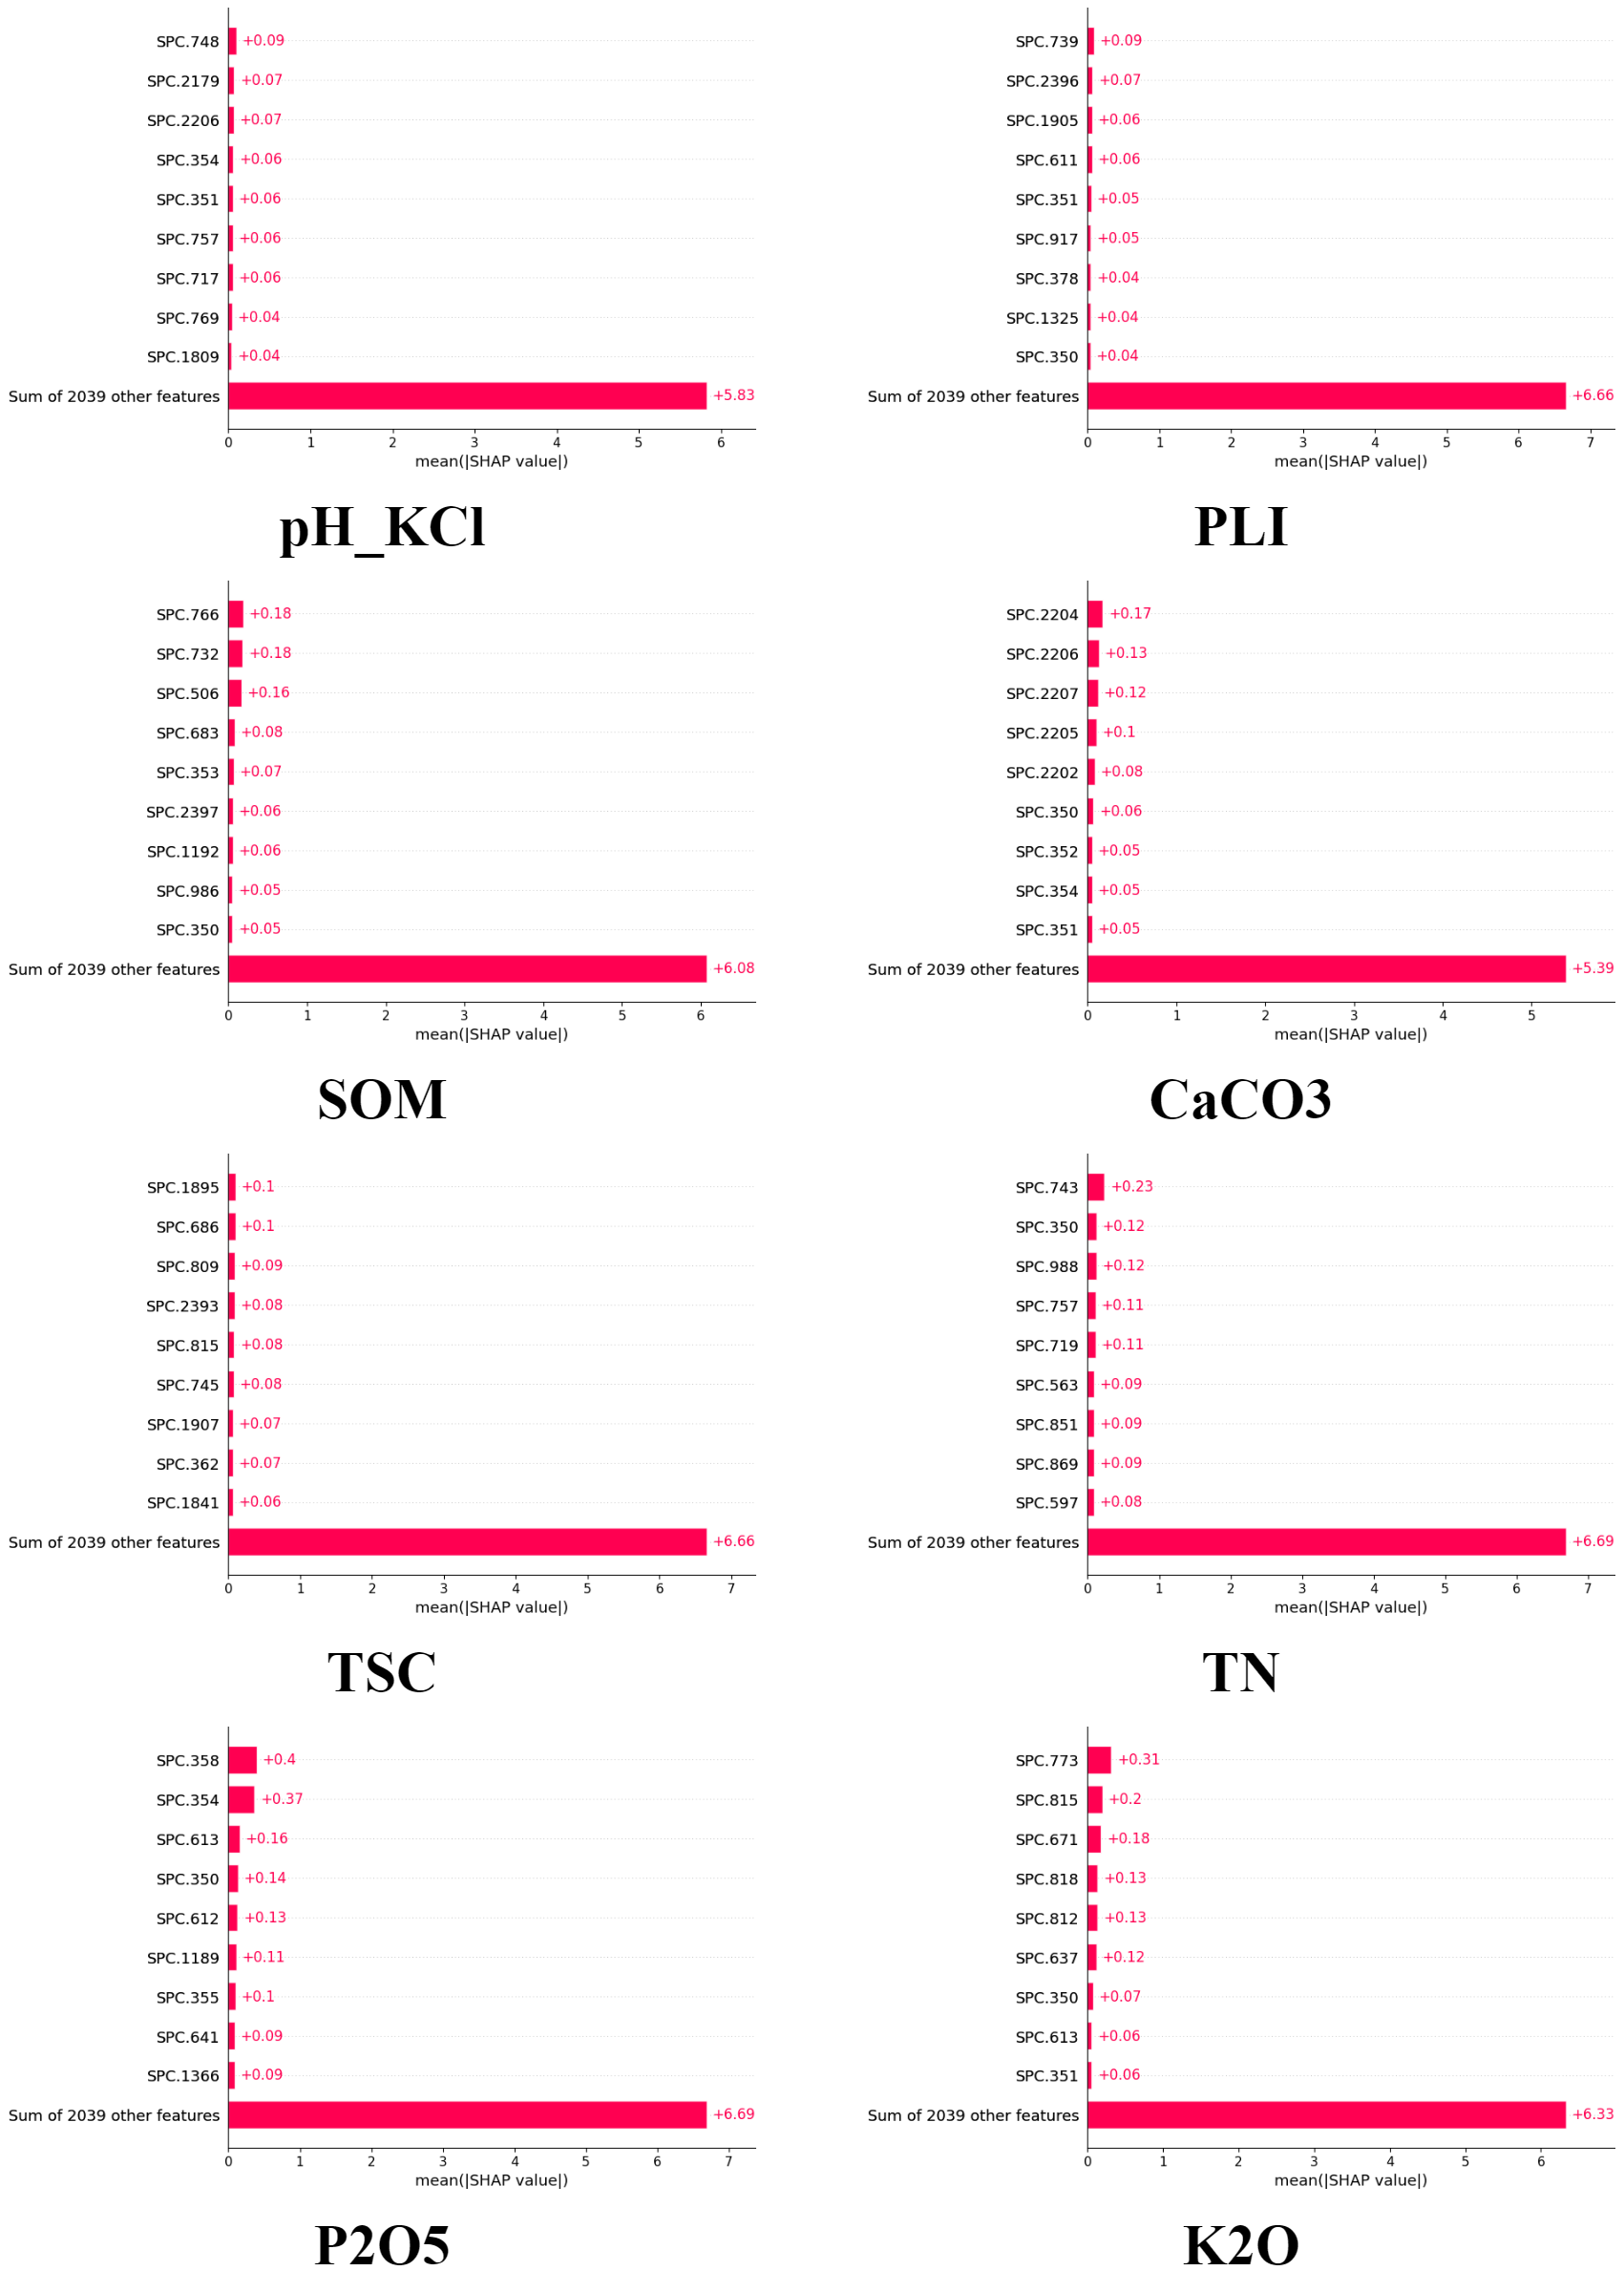
\includegraphics[width=\linewidth]{figures/Fig7.png}
  \caption{The interpretability capability of NirMACNet with the SHAP algorithm on the Soil Spectral Dataset.}
  \label{fig:figure7}
\end{figure}

Experimental evaluations conducted on two distinct datasets, one related to milk and the other to soil, demonstrate the model's robust generalization capability when applied to NIR spectral data. These results suggest that the proposed model is not only effective within the specific domains tested but also holds significant promise for broader applicability across a range of fields, including but not limited to fruit quality assessment and pharmaceutical content analysis. Furthermore, the model’s predictive performance is shown to be highly contingent upon the presence of key spectral regions within the input data, which regions are identified as having the most substantial influence on prediction outcomes \cite{phan2025ebar}. The absence or attenuation of such influential spectral features may lead to a notable decline in predictive accuracy, underscoring the critical importance of spectral region relevance in model deployment.

\section{Conclusion}\label{sec4}
This proposes a novel NirMACNet architecture for milk composition prediction using NIR spectroscopy. This model incorporates two key innovations. Firstly, residual learning blocks are integrated within the CNN architecture to address the degradation problem commonly encountered in deep neural networks. This technique facilitates the learning of deeper features and prevents performance decline as the network depth increases. Secondly, a multiscale architecture is introduced for feature extraction. This allows the model to capture information from the NIR spectra at various scales, leading to a more comprehensive understanding of the underlying data. To evaluate the effectiveness of the proposed model, we compared its performance with MLP, KAN, and a variant of the proposed model without the multiscale architecture. All models were trained and tested on the same NIR spectral dataset of milk samples.
 
The results demonstrate the superiority of the proposed NirMACNet architecture. It achieves outstanding performance in predicting milk and soil composition directly from NIR spectra, signifying its capability for end-to-end composition prediction. Furthermore, the model exhibits notable robustness under non-ideal conditions, which can be attributed to the integration of residual learning and multiscale feature extraction strategies. This work holds significant promise for various real-world applications beyond the prediction of milk and soil composition. In particular, the proposed framework can be potentially applied to a wide range of food products, including meat, fish, vegetables, and fruits, thereby broadening its impact across multiple sectors such as agriculture, food quality monitoring, and pharmaceuticals.

Future research directions will include expanding the dataset to encompass a more diverse and representative set of samples, potentially accounting for human-induced chemical interactions that may affect spectral properties. Additionally, efforts will be made to improve the model’s computational efficiency and scalability to facilitate practical deployment. In this regard, future work may also explore advanced model compression techniques, such as pruning, quantization, and architectural simplification, to enable real-time inference on edge devices or portable NIR sensors, which are commonly utilized in agricultural and industrial environments. These developments will further enhance the model's utility and adaptability in real-world settings. 

\section{Acknowledgements}
This study is funded and implemented for the project with the number "24/HĐ-SKHCN,2023". This work is supported by the People’s Committee, Da Nang, and the University of Science and
Technology, University of Danang.

\begin{thebibliography}{100}{
\fontsize{9pt}{10pt}\selectfont
\bibitem[Acquarelli et al., 2017]{acquarelli2017convolutional} Acquarelli, J., van Laarhoven, T., Gerretzen, J., Tran, T. N., Buydens, L. M., \& Marchiori, E. (2017). Convolutional neural networks for vibrational spectroscopic data analysis. \textit{Analytica Chimica Acta}, 954, 22-31.

\bibitem[Anderson et al., 2020]{anderson2020achieving} Anderson, N. T., Walsh, K. B., Subedi, P. P., \& Hayes, C. H. (2020). Achieving robustness across season, location and cultivar for a NIRS model for intact mango fruit dry matter content. \textit{Postharvest Biology and Technology}, 168, 111202.

\bibitem{chakravartula2022use} [Chakravartula et al., 2022]
 Chakravartula, S. S. N., Moscetti, R., Bedini, G., Nardella, M., \& Massantini, R. (2022). Use of convolutional neural network (CNN) combined with FT-NIR spectroscopy to predict food adulteration: A case study on coffee. \textit{Food Control}, 135, 108816.

\bibitem[Chen et al., 2022] {chen2022rapid} Chen, J., Liu, H., Li, J., \& Wang, Y. (2022). A rapid and effective method for species identification of edible boletes: FT-NIR spectroscopy combined with ResNet. \textit{Journal of Food Composition and Analysis}, 112, 104698.

\bibitem[Cui \& Fearn, 2018]{cui2018modern} Cui, C., \& Fearn, T. (2018). Modern practical convolutional neural networks for multivariate regression: Applications to NIR calibration. \textit{Chemometrics and Intelligent Laboratory Systems}, 182, 9-20.

\bibitem[Cozzolino et al., 2007]{cozzolino2007effect} Cozzolino, D., Liu, L., Cynkar, W. U., Dambergs, R. G., Janik, L., Colby, C. B., \& Gishen, M. (2007). Effect of temperature variation on the visible and near infrared spectra of wine and the consequences on the partial least square calibrations developed to measure chemical composition. \textit{Analytica Chimica Acta}, 588(2), 224-230.

\bibitem[Debus et al., 2021]{debus2021deep}Debus, B., Parastar, H., Harrington, P., \& Kirsanov, D. (2021). Deep learning in analytical chemistry. \textit{TrAC}, 145, 116459.

\bibitem[Diaz-Olivares et al., 2023]{diaz2023near} Diaz-Olivares, J. A., van Nuenen, A., Gote, M. J., Díaz, V. F., Saeys, W., Adriaens, I., \& Aernouts, B. (2023). Near-infrared spectra dataset of milk composition in transmittance mode. \textit{Data in Brief}, 51, 109767.

\bibitem[Einarson et al., 2022]{einarson2022predicting} Einarson, K. A., Baum, A., Olsen, T. B., Larsen, J., Armagan, I., Santacoloma, P. A., \& Clemmensen, L. K. (2022). Predicting pectin performance strength using near‐infrared spectroscopic data: A comparative evaluation of 1‐D convolutional neural network, partial least squares, and ridge regression modeling. \textit{Journal of Chemometrics}, 36(2), e3348.

\bibitem[Graves \& Graves, 2012]{graves2012long} Graves, A., \& Graves, A. (2012). Long short-term memory. \textit{Supervised Sequence Labelling}, 37–45.

\bibitem[Guindo et al., 2021]{guindo2021potential} Guindo, M. L., Kabir, M. H., Chen, R., \& Liu, F. (2021). Potential of Vis-NIR to measure heavy metals in different varieties of organic-fertilizers using Boruta and deep belief network. \textit{Ecotoxicology and Environmental Safety}, 228, 112996.

\bibitem[He \& Sun, 2015]{he2015convolutional} He, K., \& Sun, J. (2015). Convolutional neural networks at constrained time cost. In \textit{Proceedings of the IEEE conference on computer vision and pattern recognition} (pp. 5353-5360).

\bibitem[Helin et al., 2022]{helin2022possible} Helin, R., Indahl, U. G., Tomic, O., \& Liland, K. H. (2022). On the possible benefits... Journal of Chemometrics, 36(2), e3374.

\bibitem[Hosseinpour-Zarnaq et al., 2023]{hosseinpour2023cnn} Hosseinpour-Zarnaq, M., Omid, M., Sarmadian, F., \& Ghasemi-Mobtaker, H. (2023). A CNN model for predicting soil properties using VIS–NIR spectral data. \textit{Environmental Earth Sciences}, 82(16), 382.

\bibitem[Khorram \& Jehbez, 2023]{khorram2023hybrid} Khorram, S., \& Jehbez, N. (2023). A hybrid CNN-LSTM approach for monthly reservoir inflow forecasting. \textit{Water Resources Management}, 37(10), 4097-4121.

\bibitem[Liashchynskyi \& Liashchynskyi, 2019]{liashchynskyi2019grid}
Liashchynskyi, P., \& Liashchynskyi, P. (2019). Grid search, random search, genetic algorithm: a big comparison for NAS. \textit{arXiv preprint arXiv:1912.06059}.

\bibitem[Liu et al., 2024]{liu2024kan} Liu, Z., Wang, Y., Vaidya, S., Ruehle, F., Halverson, J. and Solja{\v{c}}i{\'c}, M., Hou, T. Y. \& Tegmark, M. (2024). Kan: Kolmogorov-Arnold Networks. \textit{arXiv:2404.19756}.

\bibitem[Lundberg \& Lee, 2017]{lundberg2017unified} Lundberg, S. M., \& Lee, S. I. (2017). A unified approach to interpreting model predictions. \textit{NIPS}, 30.

\bibitem[Malek et al., 2018]{malek2018one} Malek, S., Melgani, F., \& Bazi, Y. (2018). One‐dimensional convolutional neural networks for spectroscopic signal regression. \textit{Journal of Chemometrics}, 32(5), e2977.

\bibitem[Marini et al., 2008]{marini2008artificial} Marini, F., Bucci, R., Magrì, A. L., \& Magrì, A. D. (2008). Artificial neural networks in chemometrics: History, examples and perspectives. \textit{Microchemical journal}, 88(2), 178-185.

\bibitem[Marini, 2009]{marini2009artificial} Marini, F. (2009). Artificial neural networks in foodstuff analyses: Trends and perspectives A review. \textit{Analytica Chimica Acta}, 635(2), 121-131.

\bibitem[Melssen et al., 1994]{melssen1994using} Melssen, W. J., Smits, J. R. M., Buydens, L. M. C., \& Kateman, G. (1994). Using artificial neural networks for solving chemical problems: Part II. Kohonen self-organising feature maps and Hopfield networks. \textit{Chemometrics and Intelligent Laboratory Systems}, 23(2), 267-291.

\bibitem[Mészáros et al., 2025]{meszaros2025vis} Mészáros, J., Kovács, Z., László, P., Vass-Meyndt, S., Koós, S., Pirkó, B., Sz{\H{u}}cs-V{\'a}s{\'a}rhelyi, N., Bakacsi, Z. and Laborczi, A. \& Pásztor, L. (2025). Vis-NIR soil spectral library of the Hungarian Soil Degradation Observation System. \textit{Scientific Data}, 12(1), 363.

\bibitem[Mishra \& Passos, 2021]{mishra2021synergistic} Mishra, P., \& Passos, D. (2021). A synergistic use of chemometrics and deep learning improved the predictive performance of near-infrared spectroscopy models for dry matter prediction in mango fruit. \textit{Chemometrics and Intelligent Laboratory Systems}, 212, 104287.

\bibitem[Mishra \& Passos, 2021]{mishra2021deep} Mishra, P., \& Passos, D. (2021). Deep chemometrics: Validation and transfer of a global deep near‐infrared fruit model to use it on a new portable instrument. \textit{Journal of Chemometrics}, 35(10), e3367.

\bibitem[Mishra \& Passos, 2021]{mishra2021realizing} Mishra, P., \& Passos, D. (2021). Realizing transfer learning for updating deep learning models of spectral data to be used in new scenarios. \textit{Chemometrics and Intelligent Laboratory Systems}, 212, 104283.

\bibitem[Mishra \& Herrmann, 2021]{mishra2021gan} Mishra, P., \& Herrmann, I. (2021). GAN meets chemometrics: segmenting spectral images with pixel2pixel image translation with conditional generative adversarial networks. \textit{Chemometrics and Intelligent Laboratory Systems}, 215, 104362.

\bibitem[Ng et al., 2019]{ng2019convolutional} Ng, W., Minasny, B., Montazerolghaem, M., Padarian, J., Ferguson, R., Bailey, S., \& McBratney, A. B. (2019). Convolutional neural network for simultaneous prediction of several soil properties using visible/near-infrared, mid-infrared, and their combined spectra. \textit{Geoderma}, 352, 251-267.

\bibitem[Ng et al., 2020]{ng2020influence} Ng, W., Minasny, B., Mendes, W. D. S., \& Demattê, J. A. M. (2020). The influence of training sample size on the accuracy of deep learning models for the prediction of soil properties with near-infrared spectroscopy data. \textit{Soil}, 6(2), 565-578.

\bibitem[Özdemir et al., 2018]{ozdemir2018quantification} Özdemir, İ. S., Dağ, Ç., Özinanç, G., Suçsoran, Ö., Ertaş, E., \& Bekiroğlu, S. (2018). Quantification of sterols and fatty acids of extra virgin olive oils by FT-NIR spectroscopy and multivariate statistical analyses. \textit{LWT}, 91, 125-132.
\bibitem[Phan et al., 2025]{phan2025ebar} Nhat, P. M., Hien, N. L. H., Toan, D. M., Hung, L. V., Binh, P., Anh, P. T., Phuong, N. T. H. \& Hieu, N. V. (2025). EBAR: A Novel Machine Learning Model for Quantifying Chemical Concentrations using NIR Spectroscopy. \textit{Journal of Universal Computer Science (JUCS)}, 31(4).

\bibitem[Smits et al., 1994]{smits1994using} Smits, J. R. M., Melssen, W. J., Buydens, L. M. C., \& Kateman, G. (1994). Using artificial neural networks for solving chemical problems: Part I. Multi-layer feed-forward networks. \textit{Chemometrics and Intelligent Laboratory Systems}, 22(2), 165-189.

\bibitem[Srivastava et al., 2015]{srivastava2015highway} Srivastava, R. K., Greff, K., \& Schmidhuber, J. (2015). Highway networks. arXiv:1505.00387.

\bibitem[Takanobu et al., 2019]{takanobu2019hierarchical} Takanobu, R., Zhang, T., Liu, J., \& Huang, M. (2019, July). A hierarchical framework for relation extraction with reinforcement learning. In \textit{Proceedings of the AAAI conference on artificial intelligence} (Vol. 33, No. 01, pp. 7072-7079).

\bibitem[Vaswani et al., 2017]{vaswani2017attention} Vaswani, A., Shazeer, N., Parmar, N., Uszkoreit, J., Jones, L., Gomez, A. N., Kaiser, {\L}. \& Polosukhin, I. (2017). Attention is all you need. \textit{Advances in neural information processing systems}, 30.

\bibitem[Yang et al., 2017]{yang2017deep} Yang, H., Hu, B., Pan, X., Yan, S., Feng, Y., Zhang, X., Yin, L., \& Hu, C. (2017). Deep belief network-based drug identification using near infrared spectroscopy. \textit{Journal of Innovative Optical Health Sciences}, 10(02), 1630011.

\bibitem[Yu et al., 2018]{yu2018deep} Yu, X., Lu, H., \& Liu, Q. (2018). Deep-learning-based regression model and hyperspectral imaging for rapid detection of nitrogen concentration in oilseed rape (Brassica napus L.) leaf. \textit{Chemometrics and Intelligent Laboratory Systems}, 172, 188-193.

\bibitem[Zhang et al., 2019]{zhang2019deepspectra} Zhang, X., Lin, T., Xu, J., Luo, X., \& Ying, Y. (2019). DeepSpectra: An end-to-end deep learning approach for quantitative spectral analysis. \textit{Analytica chimica acta}, 1058, 48-57.

\bibitem[Zhang et al., 2022]{zhang2022review} Zhang, W., Kasun, L. C., Wang, Q. J., Zheng, Y., \& Lin, Z. (2022). A review of machine learning for near-infrared spectroscopy. \textit{Sensors}, 22(24), 9764.

\bibitem[Zhu et al., 2015]{zhu2015hierarchical} Zhu, W., Miao, J., Qing, L., \& Huang, G. B. (2015, July). Hierarchical extreme learning machine for unsupervised representation learning. In \textit{2015 international joint conference on neural networks (ijcnn)} (pp. 1-8). IEEE.

\bibitem[Zihao et al., 2020]{zihao2020near} Zihao, C., Xiao-li, L., \& Fei, L. (2020). Near-infrared fault detection based on stacked regularized auto-encoder network. \textit{Chemometrics and Intelligent Laboratory Systems}, 204, 104101.
}
\end{thebibliography}
\end{document}
